% Author Name: José Areia 
% Author Contact: jose.apareia@gmail.com
% Version: 2.2.5 - 2025/04/16
% Public Repository: https://github.com/joseareia/ipleiria-thesis
% Wiki/Getting Help: https://github.com/joseareia/ipleiria-thesis/wiki

%%% Document Options %%%
\documentclass[
    language=spanish,
    school=estg,
    docstage=final,
    media=paper,
    linkcolor=red!45!black,
    chapterstyle=classic,
    coverstyle=classic
]{IPLeiriaThesis} % Refer to the Wiki for a list of available options.

%%% Document Version %%%
\DocumentVersion{1.0.0} % This is required only if the 'docstage' is set to 'working'.

%%% Document Metadata %%%
% First Author (Mandatory)
\FirstAuthor{Over Haider Castrillón Valencia}
\FirstAuthorNumber{2230455}

% Second Author (Optional)
% \SecondAuthor{Jane Smith}
% \SecondAuthorNumber{2230456}

% Third Author (Optional)
% \ThirdAuthor{July Smith}
% \ThirdAuthorNumber{2230457}

% % Supervisor (Mandatory)
\Supervisor{Gustavo Isaza Echeverry}
% \SupervisorMail{joe.smith@ipleiria.pt}
% Please provide: [Current Title, Affiliation]
% \SupervisorTitle{Gustavo Adolfo Echeverry Isaza, Universidad de Caldas} 

% Co-Supervisor (Optional)
% \CoSupervisor{Steve Smith}
% \CoSupervisorMail{steve.smith@ipleiria.pt}
% \CoSupervisorTitle{Associate Professor, Polytechnic of Leiria}

% Second Co-Supervisor (Optional)
% \SecCoSupervisor{Shak Smith}
% \SecCoSupervisorMail{shak.smith@ipleiria.pt}
% \SecCoSupervisorTitle{Associate Researcher, Computer Science \& Communication Research Centre}

% Title (Mandatory)
\Title{Segundo Parcial}

% Subtitle (Mandatory)
\Subtitle{Ciberseguridad\\Segundo parcial}

% University (Mandatory)
\University{Universidad de Caldas}

% % School (Mandatory)
\School{Facultad de Inteligencia Artificial e Ingenierías}

% Department (Mandatory)
\Department{Facultad de Inteligencia Artificial e Ingenierías}

% Degree (Mandatory)
\Degree{Ingeniería en Sistemas y Computación}

% Course (Optional)
% \Course{Offensive \& Defensive Cybersecurity}

% Thesis Theme (Mandatory)
\ThesisType{Dissertation/Project/Internship \\ \textcolor{blue}{(Erase the Non-Essential)}}

% Local & Date (Mandatory)
\Date{Manizales Caldas, \DTMmonthname{\month}~\number\day~de~\number\year}

% Academic Year 
\AcademicYear{2024/25}

%%% Loading of Glossary and Acronyms %%%
\makeglossaries
\loadglsentries{Matter/04-Glossary}
\loadglsentries[\acronymtype]{Matter/05-Acronyms}

\begin{document}

%%% Front Matter %%%
\ifthenelse{\equal{\CoverOption}{classic}}{
    \newcommand\BackgroundPicCover{%
    \put(0,0){%
    \parbox[b][\paperheight]{\paperwidth}{%
    \vfill
    \centering
    
\includegraphics[width=\paperwidth,height=\paperheight,keepaspectratio]{Figures/Theme/Cover-BG.pdf}%
    \vfill
    }}}
}{
    \newcommand\BackgroundPicCover{%
    \put(0,0){%
    \parbox[b][\paperheight]{\paperwidth}{%
    \vfill
    \centering
    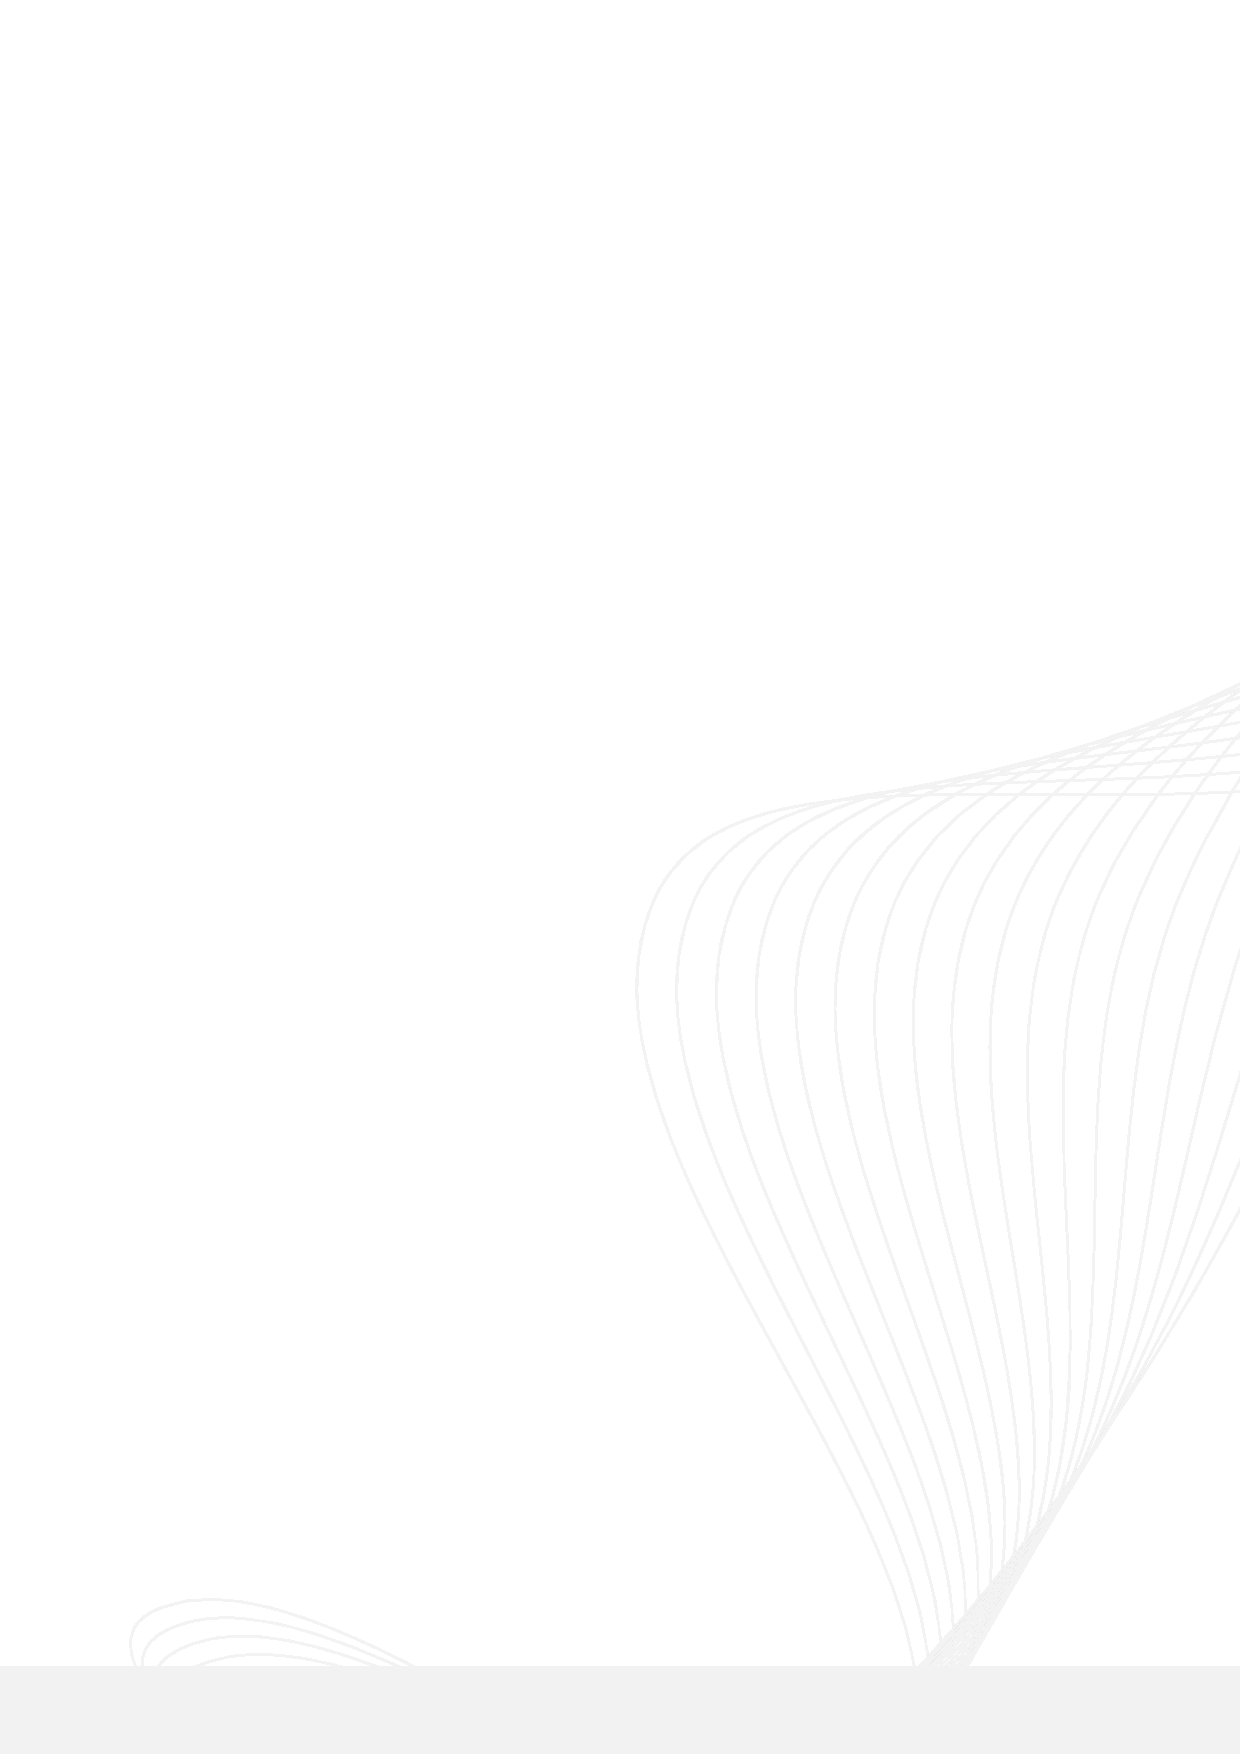
\includegraphics[width=\paperwidth,height=\paperheight,keepaspectratio]{Figures/Theme/Front-Page-BG.pdf}%
    \vfill
    }}}
}

\AddToShipoutPictureBG*{\BackgroundPicCover}

\newgeometry{margin=1.98cm, top=2.15cm, bottom=1.47cm}
\begin{titlepage}
    \latofont
    \ifthenelse{\equal{\CoverOption}{classic}}{\color{white}}{\color{frontpagedark}}
    \vspace*{\baselineskip}

    \ifthenelse{\equal{\CoverOption}{classic}}{
        \ifthenelse{\equal{\SchoolOption}{estg}}{
            \begin{figure}
                
\includegraphics[width=0.485\linewidth]{Figures/Theme/Logotypes/uc-logo-w.png}
            \end{figure}
        }{}

        
        
        \ifthenelse{\equal{\SchoolOption}{esad}}{
            \begin{figure}
                
\includegraphics[width=0.485\linewidth]{Figures/Theme/Logotypes/IPLeiria-ESAD-Logo-W.pdf}
            \end{figure}
        }{}
        
        \ifthenelse{\equal{\SchoolOption}{esslei}}{
            \begin{figure}
                
\includegraphics[width=0.485\linewidth]{Figures/Theme/Logotypes/IPLeiria-ESSLEI-Logo-W.pdf}
            \end{figure}
        }{}
        
        \ifthenelse{\equal{\SchoolOption}{estm}}{
            \begin{figure}
                
\includegraphics[width=0.485\linewidth]{Figures/Theme/Logotypes/IPLeiria-ESTM-Logo-W.pdf}
            \end{figure}
        }{}
        
        \ifthenelse{\equal{\SchoolOption}{esecs}}{
            \begin{figure}
                
\includegraphics[width=0.485\linewidth]{Figures/Theme/Logotypes/IPLeiria-ESECS-Logo-W.pdf}
            \end{figure}
        }{}

    } {
        \ifthenelse{\equal{\SchoolOption}{estg}}{
            \begin{figure}
                
\includegraphics[width=0.485\linewidth]{Figures/Theme/Logotypes/IPLeiria-ESTG-Logo-B.pdf}
                
\includegraphics[width=0.4\linewidth]{Figures/Theme/Logotypes/IPLeiria-ESTG-Logo-Old.png}
            \end{figure}
        }{}
        
        \ifthenelse{\equal{\SchoolOption}{esad}}{
            \begin{figure}
                
\includegraphics[width=0.485\linewidth]{Figures/Theme/Logotypes/IPLeiria-ESAD-Logo-B.pdf}
            \end{figure}
        }{}
        
        \ifthenelse{\equal{\SchoolOption}{esslei}}{
            \begin{figure}
                
\includegraphics[width=0.485\linewidth]{Figures/Theme/Logotypes/IPLeiria-ESSLEI-Logo-B.pdf}
            \end{figure}
        }{}
        
        \ifthenelse{\equal{\SchoolOption}{estm}}{
            \begin{figure}
                
\includegraphics[width=0.485\linewidth]{Figures/Theme/Logotypes/IPLeiria-ESTM-Logo-B.pdf}
            \end{figure}
        }{}
        
        \ifthenelse{\equal{\SchoolOption}{esecs}}{
            \begin{figure}
                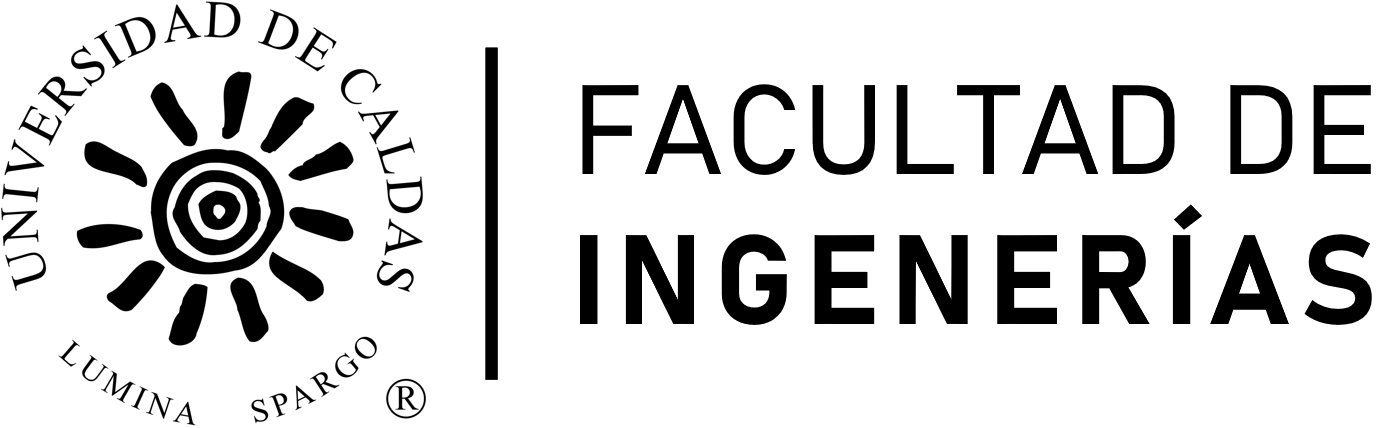
\includegraphics[width=0.485\linewidth]{Figures/Theme/Logotypes/uc-logo-b.png}
            \end{figure}
        }{}
    }

    \vspace{5.5\baselineskip}

    % Title.
	\noindent
    \makebox[\textwidth][l]{%
        \parbox{\dimexpr\textwidth-4cm\relax}{
            \setstretch{1.03}
            \raggedright\bfseries\fontsize{20}{26}\selectfont\GetTitle
        }
    }

    \vspace{0.8\baselineskip}

    % Subtitle.
    \noindent
    \makebox[\textwidth][l]{%
        \parbox{\dimexpr\textwidth-7cm\relax}{
            \setstretch{1.03}
            \raggedright\fontsize{14}{19}\selectfont\GetSubtitle
        }
    }

    \vspace{35pt}  

    % Author.
    {\noindent\bfseries\fontsize{14}{19}\selectfont\GetFirstAuthor}

    \ifdefined\GetSecondAuthor
        \vspace{8pt}
        {\noindent\bfseries\fontsize{14}{19}\selectfont\GetSecondAuthor}
	\fi

    \ifdefined\GetThirdAuthor
        \vspace{8pt}
        {\noindent\bfseries\fontsize{14}{19}\selectfont\GetThirdAuthor}
	\fi
 
	\vfill

    % School.
	{\noindent\fontsize{10}{12}\selectfont\GetSchool}
	
    % Department.
	{\noindent\fontsize{10}{12}\selectfont\GetDepartment}

    % Degree.
	{\noindent\fontsize{10}{12}\selectfont\GetDegree}

    % Course.
    \ifdefined\GetCourse
        {\noindent\fontsize{10}{12}\selectfont\GetCourse}
	\fi

    \ifthenelse{\equal{\DocStageOption}{working}}{
        \vspace{62pt}
        {\noindent\fontsize{10}{12}\selectfont\overwritecolor{yellow}{\GetDocumentVersion \\ \textit{\today}}} 
        \vspace{62pt}
    }{
        \vspace{125pt}
    }

    % Local & Date.
	{\noindent\fontsize{10}{12}\selectfont\GetDate}

    \vspace{68pt}
\end{titlepage}
\restoregeometry
\MediaOptionLogicBlank
\newcommand\BackgroundPicFrontPage{%
    \put(0,0){%
    \parbox[b][\paperheight]{\paperwidth}{%
    \vfill
    \centering
    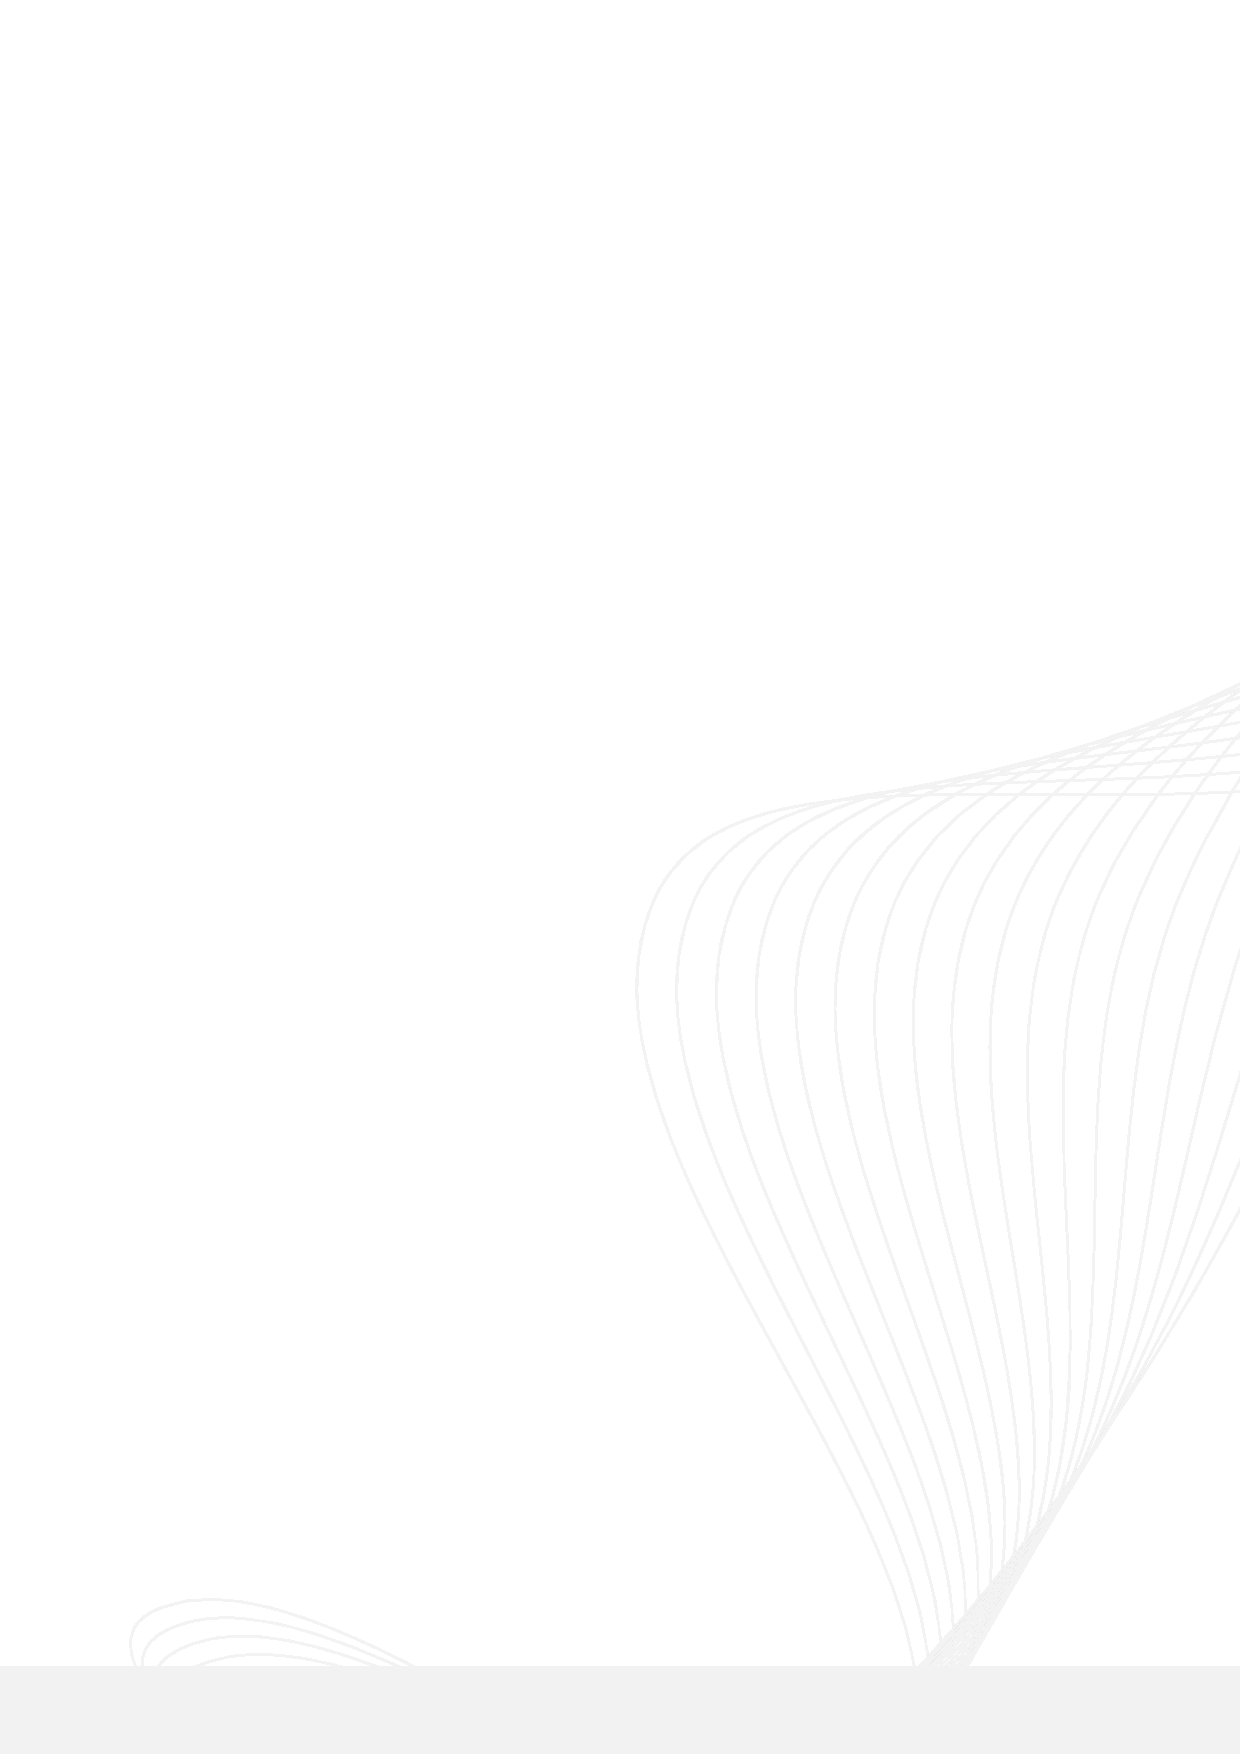
\includegraphics[width=\paperwidth,height=\paperheight,keepaspectratio]{Figures/Theme/Front-Page-BG.pdf}%
    \vfill
}}}
\AddToShipoutPictureBG*{\BackgroundPicFrontPage}

\newgeometry{margin=1.98cm, top=2.15cm, bottom=1.47cm}
\begin{titlepage}
    \latofont
    \color{frontpagedark}
    \vspace*{\baselineskip}

    \ifthenelse{\equal{\SchoolOption}{estg}}{
        \begin{figure}
            % 
\includegraphics[width=0.485\linewidth]{Figures/Theme/Logotypes/IPLeiria-ESTG-Logo-B.pdf}
            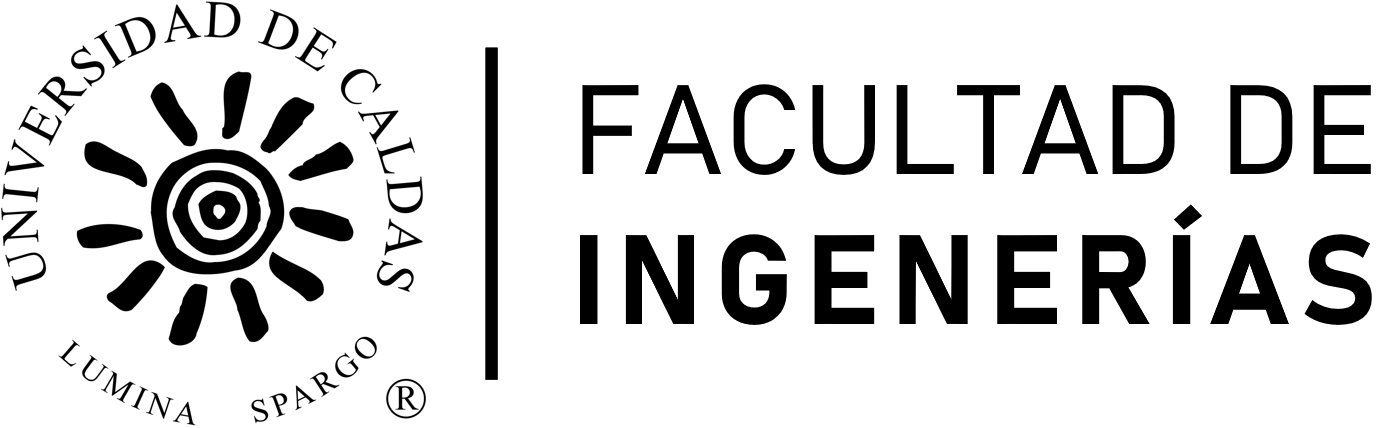
\includegraphics[width=0.4\linewidth]{Figures/Theme/Logotypes/uc-logo-b.png}
        \end{figure}
    }
    
    % \ifthenelse{\equal{\SchoolOption}{esad}}{
    %     \begin{figure}
    %         
\includegraphics[width=0.485\linewidth]{Figures/Theme/Logotypes/IPLeiria-ESAD-Logo-B.pdf}
    %     \end{figure}
    % }
    
    % \ifthenelse{\equal{\SchoolOption}{esslei}}{
    %     \begin{figure}
    %         
\includegraphics[width=0.485\linewidth]{Figures/Theme/Logotypes/IPLeiria-ESSLEI-Logo-B.pdf}
    %     \end{figure}
    % }
    
    % \ifthenelse{\equal{\SchoolOption}{estm}}{
    %     \begin{figure}
    %         
\includegraphics[width=0.485\linewidth]{Figures/Theme/Logotypes/IPLeiria-ESTM-Logo-B.pdf}
    %     \end{figure}
    % }
    
    % \ifthenelse{\equal{\SchoolOption}{esecs}}{
    %     \begin{figure}
    %         
\includegraphics[width=0.485\linewidth]{Figures/Theme/Logotypes/IPLeiria-ESECS-Logo-B.pdf}
    %     \end{figure}
    % }

    \vspace{3.5\baselineskip}

    % Title.
	\noindent
    \makebox[\textwidth][l]{%
        \parbox{\dimexpr\textwidth-2.5cm\relax}{
            \setstretch{1.03}
            \raggedright\bfseries\fontsize{20}{26}\selectfont\GetTitle
        }
    }

    \vspace{0.8\baselineskip}

    % Subtitle.
    % \noindent
    % \makebox[\textwidth][l]{%
    %     \parbox{\dimexpr\textwidth-7cm\relax}{
    %         \setstretch{1.03}
    %         \raggedright\fontsize{14}{19}\selectfont\GetSubtitle
    %     }
    % }

    \vspace{35pt}

    % Author.
    {\noindent\bfseries\fontsize{14}{19}\selectfont\GetFirstAuthor}

    \ifdefined\GetSecondAuthor
        \vspace{8pt}
        {\noindent\bfseries\fontsize{14}{19}\selectfont\GetSecondAuthor}
	\fi

    \ifdefined\GetThirdAuthor
        \vspace{8pt}
        {\noindent\bfseries\fontsize{14}{19}\selectfont\GetThirdAuthor}
	\fi

    \vspace{70pt}    

    {
    \noindent
    \latofont
    \fontsize{10}{12}\selectfont
    \renewcommand{\arraystretch}{0.1}
    \hspace*{-2.5pt}\begin{tabular}{@{}r@{\hspace{5pt}}>{\raggedright\arraybackslash}m{6cm}@{}}
        \textbf{Docente:} & \GetSupervisor \\ [-.7ex]
        & \setstretch{0.9}{\fontsize{8}{10}\selectfont\itshape \GetSupervisorTitle} \\ [2ex]
        
        \ifdefined\GetCoSupervisor
            \textbf{Co-supervisor:} & \GetCoSupervisor \\ [-.7ex]
            & \setstretch{0.9}{\fontsize{8}{10}\selectfont\itshape \GetCoSupervisorTitle} \\ [.5ex]
        \fi

        \ifdefined\GetSecCoSupervisor        
            & \GetSecCoSupervisor \\ [-.7ex]
            & \setstretch{0.9}{\fontsize{8}{10}\selectfont\itshape \GetSecCoSupervisorTitle} \\
        \fi
    \end{tabular}
    }
    
    \vfill
	
    % School.
	{\noindent\fontsize{10}{12}\selectfont\GetSchool}
	
    % Department.
	{\noindent\fontsize{10}{12}\selectfont\GetDepartment}

    % Degree.
	{\noindent\fontsize{10}{12}\selectfont\GetDegree}

    % Course.
    \ifdefined\GetCourse
        {\noindent\fontsize{10}{12}\selectfont\GetCourse}
	\fi

    \vspace{45pt}

    % Thesis option.
	% {\noindent\fontsize{10}{12}\itshape\selectfont\GetThesisType}

    \vspace{45pt}

    % Local and date.
	{\noindent\fontsize{10}{12}\selectfont\GetDate}

    \vspace{68pt}
\end{titlepage}
\restoregeometry
\MediaOptionLogicBlank

%%% Copyright Statement %%%
% \pagenumbering{gobble} % Prevent page numbering.

\vspace*{\fill}

\ifthenelse{\equal{\LanguageOption}{portuguese}}{%
    \noindent \textbf{\GetTitle}
    
    \noindent Copyright \textcopyright~\the\year{} - \GetFirstAuthor, \GetSchool.
    
    \vspace{.575em}
    
    \noindent A presente dissertação é um trabalho original, elaborado exclusivamente para este fim, tendo sido devidamente citados todos os autores cujos estudos contribuíram para a sua elaboração. É permitida a sua reprodução parcial com indicação do autor e referência ao grau, ano letivo, instituição---\textit{Politécnico de Leiria}---e data da defesa pública.

    \vspace{1.395em}
    
    \noindent\psvectorian[scale=.25,opacity=.80]{2}
    
    \vspace{.935em}

    \noindent O presente trabalho beneficiou da utilização do modelo \textit{IPLeiria-Thesis}.
}{%
    \noindent \textbf{\GetTitle}
    
    \noindent Copyright \textcopyright~\the\year{} - \GetFirstAuthor, \GetSchool.
    
    \vspace{.575em}
    
    \noindent This dissertation is original work, written solely for this purpose, and all the authors whose studies and publications contributed to it have been duly cited. Partial reproduction is allowed with acknowledgment of the author and reference to the degree, academic year, institution---\textit{Polytechnic University of Leiria}---and public defense date.

    \vspace{1.395em}
    
    \noindent\psvectorian[scale=.25,opacity=.80]{2}
    
    \vspace{.935em}

    \noindent Preparation of this work was facilitated by the use of the \textit{IPLeiria-Thesis} template.
}

\vspace*{\fill}
\MediaOptionLogic

%%% Roman Numeration %%%
\pagenumbering{roman}

%%% Acknowledgements %%%
% \ifthenelse{\equal{\LanguageOption}{portuguese}}{%
%     \chapter*{Agradecimentos}
% }{%
%     \chapter*{Acknowledgements}
% }

% \guideinfo{In the \textit{Acknowledgment} section, express your gratitude to those who helped and supported your work. Start by thanking your advisors, mentors, or supervisors who provided guidance and expertise. Mention any colleagues, classmates, or team members who contributed to discussions or offered assistance. You can also acknowledge specific organisations, institutions, or funding sources that supported your research or work. Lastly, include any personal acknowledgments for family or friends who offered encouragement and moral support during the project. Keep this section sincere, concise, and professional.}

% \MediaOptionLogicBlank

%%% Abstract %%%
% \thispagestyle{plain}
% \chapter*{Resumo}

% \guiainfo{Na secção \textit{Resumo}, apresente um resumo conciso do seu projeto, destacando os pontos principais. Comece com uma breve declaração do problema ou objetivo, seguido de uma descrição da sua abordagem ou metodologia. Resuma os principais resultados ou conclusões, salientando a sua importância ou implicações. Conclua com uma ou duas frases sobre a contribuição global ou o impacto do seu trabalho. O resumo deve ser claro e conciso, idealmente com 150-250 palavras, para que os leitores compreendam rapidamente o seu trabalho e a sua importância.}

% \keywordspt{Palavra-Chave A, Palavra-Chave B, Palavra-Chave C.}

% \MediaOptionLogicBlank

% \pdfbookmark[1]{Abstract}{abstract}
% \chapter*{Abstract}
% \guideinfo{In the \textit{Abstract} section, provide a concise summary of your project, highlighting the key points. Begin with a brief statement of the problem or objective, followed by a description of your approach or methodology. Summarise the main results or findings, emphasising their significance or implications. Conclude with a sentence or two on the overall contribution or impact of your work. Keep the abstract clear and focused, ideally within 150-250 words, to give readers a quick understanding of your research and its importance.}

% \keywordsen{Keyword A, Keyword B, Keyword C.}

% \MediaOptionLogicBlank

% %%% Table of Contents, List of Figures and List of Tables %%%
\bookmarktocentry\tableofcontents
% \listoffigures
% \listoftables

%%% Print: Glossary and Acronyms %%%
% \glossarytoc\printnormalglossary
% \acronymtoc\printacronymglossary

%%% Arabic Numeration %%%
\pagenumbering{arabic}

%%% Chapters (**Insert Yours Here**) %%%
\chapter[Planteamientos]{Planteamientos}
% \label{cp:introduction}

{
\parindent0pt


% \textit{Official Repository: \href{https://github.com/joseareia/ipleiria-thesis}{GitHub Repository}}

\vspace{.935em}

\section{Problema 1 (25\%)}

\subsection{Literal a}
Aplicando Criptoanálisis por factorización, especifique el proceso y determine el PlainText (P) del siguiente Criptograma RSA (puede usar WolframAlpha para funciones exponenciales):

\begin{itemize}[leftmargin=*]
    \item $p=19$, $q=67$
    \item $KU=(5,1273)$
    \item Criptograma: $1252-1079-319-337-231-1100-507-1100-231-213-192$
\end{itemize}

\textbf{Algoritmo AEE (n, a):}
\begin{lstlisting}[basicstyle=\ttfamily]
Hacer (g0, g1, u0, u1, v0, v1, i) = (n, a, 1, 0, 0, 1, 1)
Mientras gi distinto 0 hacer
    Hacer yi+1 = parte entera (gi-1/gi)
    Hacer gi+1 = gi-1 - yi+1 × gi
    Hacer ui+1 = ui-1 - yi+1 × ui
    Hacer vi+1 = vi-1 - yi+1 × vi
    Hacer i = i+1
Si (vi-1 < 0)
    Hacer vi-1 = vi-1 + n
Hacer x = vi-1
\end{lstlisting}




\textbf{Solución:}


Se nos proporciona la siguiente información:

\begin{itemize}
\item $n = 1273$
\item $p = 19$
\item $q = 67$
\item $d = 5$
\item $z = (p-1)(q-1) = (19-1)(67-1) = 1188$
\end{itemize}

Y el siguiente mensaje cifrado:

\begin{verbatim}
1252 1079 319 337 231
1100 507 1100 231 213
192
\end{verbatim}

\subsubsection{Cálculo del inverso multiplicativo módulo $z$}

Necesitamos encontrar $e$ tal que $e \cdot d \equiv 1 ~mod~z$, es decir, el inverso multiplicativo de $d$ módulo $z$.

Para ello utilizaremos el algoritmo de Euclides extendido:

\textbf{Inicialización del algoritmo:}

Estamos buscando $e$ tal que $e \cdot 5 \equiv 1 ~\text{mod}~{1188}$

Inicializamos las variables según el algoritmo:

$$g_0 = 1188, g_1 = 5$$
$$u_0 = 1, u_1 = 0$$
$$v_0 = 0, v_1 = 1$$



\textbf{Iteración 1:}

Calculamos $y_2 = \lfloor g_0 / g_i \rfloor = \lfloor 1188 / 5 \rfloor = 237$

Calculamos $g_2 = g_0 - y_2 \cdot g_i = 1188 - 237 \cdot 5 = 3$

Calculamos $u_2 = u_0 - y_2 \cdot u_i = 1 - 237 \cdot 0 = 1$

Calculamos $v_2 = v_0 - y_2 \cdot v_i = 0 - 237 \cdot 1 = -237$



\textbf{Iteración 2:}

Calculamos $y_3 = \lfloor g_1 / g_i \rfloor = \lfloor 5 / 3 \rfloor = 1$

Calculamos $g_3 = g_1 - y_3 \cdot g_i = 5 - 1 \cdot 3 = 2$

Calculamos $u_3 = u_1 - y_3 \cdot u_i = 0 - 1 \cdot 1 = -1$

Calculamos $v_3 = v_1 - y_3 \cdot v_i = 1 - 1 \cdot -237 = 238$



\textbf{Iteración 3:}
Calculamos $y_4 = \lfloor g_2 / g_i \rfloor = \lfloor 3 / 2 \rfloor = 1$

Calculamos $g_4 = g_2 - y_4 \cdot g_i = 3 - 1 \cdot 2 = 1$

Calculamos $u_4 = u_2 - y_4 \cdot u_i = 1 - 1 \cdot -1 = 2$

Calculamos $v_4 = v_2 - y_4 \cdot v_i = -237 - 1 \cdot 238 = -475$



\textbf{Iteración 4:}

Calculamos $y_5 = \lfloor g_3 / g_i \rfloor = \lfloor 2 / 1 \rfloor = 2$

Calculamos $g_5 = g_3 - y_5 \cdot g_i = 2 - 2 \cdot 1 = 0$

Calculamos $u_5 = u_3 - y_5 \cdot u_i = -1 - 2 \cdot 2 = -5$

Calculamos $v_5 = v_3 - y_5 \cdot v_i = 238 - 2 \cdot -475 = 1188$



\textbf{Resultado final:}

El algoritmo ha terminado porque $g_4 = 0$

El inverso se encuentra en el valor de $v$ en el penúltimo paso: $v_3 = -475$

Como $v_3 < 0$, ajustamos: $v_3 = v_3 + B = -475 + 1188 = 713$

Por lo tanto, el inverso multiplicativo de 5 módulo 1188 es 713

Verificación: $5 \cdot 713 \equiv 1 ~\text{mod}~1188$

\begin{table}[h]
\centering
\begin{tabular}{|c|c|c|c|c|}
\hline
$i$ & $y_i$ & $g_i$ & $u_i$ & $v_i$ \\ \hline
0 & - & 1188 & 1 & 0 \\ \hline
1 & - & 5 & 0 & 1 \\ \hline
2 & 237 & 3 & 1 & -237 \\ \hline
3 & 1 & 2 & -1 & 238 \\ \hline
4 & 1 & 1 & 2 & -475 \\ \hline
5 & 2 & 0 & -5 & 1188 \\ \hline
\end{tabular}
\caption{Cálculo del inverso modular utilizando el algoritmo de Euclides extendido}
\label{tab:euclides}
\end{table}

Por lo tanto $e = 713$.

\subsubsection{Descifrado del mensaje}

Para descifrar el mensaje, utilizamos la fórmula $M = C^e ~\text{mod}~ n$, donde $e = 713$ y $n = 1273$.

\subsubsection{Proceso de descifrado}

$C = 1252: M = 1252^{713} ~\text{mod}~ 1273 = 80$ (ASCII: 'P')

$C = 1079: M = 1079^{713} ~\text{mod}~ 1273 = 117$ (ASCII: 'u')

$C = 319: M = 319^{713} ~\text{mod}~ 1273 = 98$ (ASCII: 'b')

$C = 337: M = 337^{713} ~\text{mod}~ 1273 = 108$ (ASCII: 'l')

$C = 231: M = 231^{713} ~\text{mod}~ 1273 = 105$ (ASCII: 'i')

$C = 1100: M = 1100^{713} ~\text{mod}~ 1273 = 99$ (ASCII: 'c')

$C = 507: M = 507^{713} ~\text{mod}~ 1273 = 97$ (ASCII: 'a')

$C = 1100: M = 1100^{713} ~\text{mod}~ 1273 = 99$ (ASCII: 'c')

$C = 231: M = 231^{713} ~\text{mod}~ 1273 = 105$ (ASCII: 'i')

$C = 213: M = 213^{713} ~\text{mod}~ 1273 = 111$ (ASCII: 'o')

$C = 192: M = 192^{713} ~\text{mod}~ 1273 = 110$ (ASCII: 'n')

\begin{table}[h]
\centering
\begin{tabular}{|c|c|c|}
\hline
$C$ & $M$ & ASCII \\ \hline
1252 & 80 & 'P' \\ \hline
1079 & 117 & 'u' \\ \hline
319 & 98 & 'b' \\ \hline
337 & 108 & 'l' \\ \hline
231 & 105 & 'i' \\ \hline
1100 & 99 & 'c' \\ \hline
507 & 97 & 'a' \\ \hline
1100 & 99 & 'c' \\ \hline
231 & 105 & 'i' \\ \hline
213 & 111 & 'o' \\ \hline
192 & 110 & 'n' \\ \hline
\end{tabular}
\caption{Descifrado RSA: $m = c^e ~\text{mod}~ n$}
\label{tab:descifrado}
\end{table}

\subsubsection{Mensaje descifrado}

El mensaje descifrado es:

\begin{verbatim}
Publicacion
\end{verbatim}





\pagebreak
\subsection{Literal b}
¿En qué principios \textit{(al menos 2)} reposa la seguridad de RSA?

\textbf{Respuesta:}
\begin{itemize}
    \item La gran dificultad computacional que hay inscrita en el problema de la factorización de números enteros grandes.
    \item La complejidad del problema del logaritmo discreto.
    \item La función de una vía con trampa (trapdoor) que permite cifrar fácilmente pero descifrar solo con información "privilegiada".
\end{itemize}

\subsection{Literal c}
¿Por qué la Criptografía de Curvas Elípticas es una opción viable para los retos Crypto actuales?

\textbf{Respuesta:}

En efecto maestro, la Criptografía de Curvas Elípticas (ECC) es una opción viable porque:
\begin{itemize}
    \item Ofrece el mismo nivel de seguridad que el RSA pero ya con claves de un menor tamaño.
    \item Hay menor consumo de recursos computacionales.
    \item Tiene una mayor eficiencia en dispositivos con recursos limitados.
    \item Presenta mayor resistencia a los ataques cuánticos en comparación con RSA.
\end{itemize}

\section{Problema 2 (25\%)}

\subsection{Literal a}
En el marco de la Seguridad Ofensiva, describa la secuencia para verificar y explotar una vulnerabilidad de acceso remoto a un host (tipo Win o Linux) y describa alguna estrategia de uso en un proceso de "Hacking Ético".


\textbf{Respuesta:}
La secuencia para verificar y explotar una vulnerabilidad de acceso remoto sigue un proceso metodológico conocido como "Cyber Kill Chain" o ciclo de ataque, que en el contexto de hacking ético permite identificar, evaluar y documentar vulnerabilidades de forma sistemática:

\begin{enumerate}
    \item \textbf{Obtención de Información (Reconocimiento):} 
    \begin{itemize}
        \item Recopilación de datos sobre el objetivo mediante técnicas OSINT.
        \item \textit{Herramientas:} Usenet, whois, dig, nslookup, dnsmap, fierce, DNSPredict.
        \item Enfoque ético: Limitarse a fuentes públicas y obtener autorización previa.
    \end{itemize}

    \item \textbf{Escaneo:} 
    \begin{itemize}
        \item Identificación de hosts activos, puertos abiertos y servicios en ejecución.
        \item Detección de sistemas operativos y versiones de software.
        \item \textit{Herramientas:} Fping, hping, nmap, SuperScan, AutoScan, xprobe2, Nessus.
        \item Enfoque ético: Realizar escaneos en horarios de bajo impacto y con notificación previa.
    \end{itemize}

    \item \textbf{Enumeración:} 
    \begin{itemize}
        \item Obtención de usuarios, grupos, recursos compartidos y configuraciones.
        \item \textit{Herramientas:} DumpSec, NmbSscan, Telnet, NetCat, rpcinfo, snmpenum.
        \item Enfoque ético: Documentar meticulosamente cada hallazgo sin explotar información sensible.
    \end{itemize}

    \item \textbf{Obtención de Acceso:} 
    \begin{itemize}
        \item Explotación de vulnerabilidades identificadas para obtener acceso inicial.
        \item \textit{Herramientas:} Airsnarf, dsniff, Metasploit Framework.
        \item Enfoque ético: Limitar el impacto de la explotación y documentar cada acción.
    \end{itemize}

    \item \textbf{Escalamiento de Privilegios:} 
    \begin{itemize}
        \item Elevación de permisos para obtener control administrativo del sistema.
        \item \textit{Herramientas:} John the Ripper, LCP, rcrack, ophcrack, Cain\&Abel, Metasploit Framework.
        \item Enfoque ético: Utilizar técnicas que no comprometan la estabilidad del sistema.
    \end{itemize}

    \item \textbf{Hurto o Exfiltración de Información:} 
    \begin{itemize}
        \item Simulación de extracción de datos sensibles para demostrar el impacto.
        \item \textit{Herramientas:} Rhosts, Config Files, Cain \& Abel.
        \item Enfoque ético: No extraer datos reales; utilizar marcadores o datos de prueba.
    \end{itemize}

    \item \textbf{Cubrimiento de Pistas:} 
    \begin{itemize}
        \item Análisis de logs y rastros digitales.
        \item \textit{Herramientas:} Logclean-ng, wtmpclean, rootkits, dataflows.
        \item Enfoque ético: Documentar todas las modificaciones realizadas para facilitar la restauración.
    \end{itemize}

    \item \textbf{Creación de Puertas Traseras:} 
    \begin{itemize}
        \item Demostración de cómo un atacante podría mantener acceso persistente.
        \item \textit{Herramientas:} Cron, Register Keys, Netcat, psexec, keyloggers, fwpclnt.dll, ps, netstat.
        \item Enfoque ético: Eliminar completamente cualquier puerta trasera al finalizar las pruebas.
    \end{itemize}
\end{enumerate}

\textbf{Estrategia de uso en un proceso de Hacking Ético:}

Una estrategia efectiva para implementar estas fases en un proceso de hacking ético incluye:

\begin{itemize}
    \item \textbf{Definición clara del alcance:} Establecemos los límites específicos y objetivos de la evaluación mediante un acuerdo formal (Rules of Engagement).
    
    \item \textbf{Enfoque de caja negra, gris o blanca:} Adaptamos la metodología según el nivel de información previa disponible sobre el objetivo.
    
    \item \textbf{Documentación exhaustiva:} Registramos meticulosamente cada paso, herramienta, hallazgo y recomendación para facilitar la remediación.
    
    \item \textbf{Prueba de concepto (PoC) controlada:} Demostramos las vulnerabilidades con impacto mínimo y sin afectar operaciones críticas.
    
    \item \textbf{Comunicación continua:} Mantenemos informados a los responsables del sistema, especialmente ante hallazgos críticos que requieran atención inmediata.
    
    \item \textbf{Análisis de impacto:} Evaluamos cada vulnerabilidad en función de la criticidad, facilidad de explotación e impacto potencial en el negocio.
    
    \item \textbf{Recomendaciones priorizadas:} Proporcionamos soluciones que sean prácticas y priorizamos la mitigación de esas vulnerabilidades encontradas.
\end{itemize}

Con este enfoque podemos identificar y documentar vulnerabilidades de forma sistemática, proporcionando una base sólida para mejorar la postura de seguridad de la organización.





\subsection{Literal b}
Enumere al menos 3 controles (de un estándar, normativa o Sistema de Gestión de Seguridad de la Información), que puedan implementarse posterior a un proceso de Seguridad Ofensiva, como estrategia preventiva.

\textbf{Respuesta:}

\begin{enumerate}
    \item \textbf{ISO/IEC 27001:2013 - Anexo A}
    \begin{itemize}
        \item \textbf{A.12.6.1 Gestión de las vulnerabilidades técnicas}: Este control requiere que se obtenga información oportuna sobre vulnerabilidades técnicas de los sistemas de información, se evalúe la exposición de la organización a dichas vulnerabilidades y se tomen medidas apropiadas para abordar los riesgos asociados.
        
        \textit{Aplicación post-seguridad ofensiva}: Tras un pentesting o evaluación ofensiva, este control permite establecer un proceso sistemático para abordar las vulnerabilidades descubiertas, priorizarlas según su criticidad e implementar las correcciones necesarias. Incluye la creación de un inventario preciso de activos tecnológicos, la suscripción a servicios de alertas de vulnerabilidades y la implementación de procedimientos regulares de parcheo.
        
        \item \textbf{A.9.4.2 Procedimientos seguros de inicio de sesión}: Establece que el acceso a los sistemas y aplicaciones debe estar controlado por procedimientos seguros de inicio de sesión.
        
        \textit{Aplicación post-seguridad ofensiva}: Después de que las pruebas de intrusión revelen debilidades en los mecanismos de autenticación, este control impulsa la implementación de técnicas robustas como limitación de intentos fallidos, registro detallado de accesos, tiempo de espera para sesiones inactivas, y no mostrar identificadores de sistema hasta que el proceso de inicio de sesión se haya completado exitosamente.
        
        \item \textbf{A.13.1.3 Segregación en redes}: Indica que los grupos de servicios de información, usuarios y sistemas deben estar segregados en redes diferentes.
        
        \textit{Aplicación post-seguridad ofensiva}: Cuando las evaluaciones de seguridad revelan problemas de movimiento lateral o elevación de privilegios, este control permite implementar arquitecturas de red segmentadas con firewalls internos, zonas desmilitarizadas (DMZ) y redes VLAN separadas por funciones, limitando el impacto potencial de una brecha de seguridad.
    \end{itemize}

    \item \textbf{NIST SP 800-53 Rev. 5}
    \begin{itemize}
        \item \textbf{SI-7 Integridad del software, firmware y la información}: Requiere que la organización emplee herramientas para detectar cambios no autorizados en software, firmware e información.
        
        \textit{Aplicación post-seguridad ofensiva}: Tras identificar manipulaciones o inyecciones durante pruebas ofensivas, este control permite implementar mecanismos de verificación de integridad como sumas de comprobación, firmas digitales y monitoreo en tiempo real para detectar alteraciones no autorizadas en archivos críticos del sistema o aplicaciones.
        
        \item \textbf{AC-6(1) Privilegio mínimo - Autorizar acceso a funciones de seguridad}: Especifica que la organización debe autorizar explícitamente el acceso a funciones específicas de seguridad y a información relacionada con la seguridad.
        
        \textit{Aplicación post-seguridad ofensiva}: Cuando las pruebas revelan exceso de privilegios o controles de acceso débiles, este control permite implementar una estrategia rigurosa de privilegio mínimo, separando cuentas administrativas de cuentas regulares, empleando sistemas de gestión de acceso privilegiado (PAM) y requiriendo autorizaciones específicas para acceder a funciones de seguridad críticas.
        
        \item \textbf{SC-7(10) Protección de límites - Prevenir tráfico saliente no autorizado}: Requiere que el sistema de información impida la exfiltración no autorizada de información.
        
        \textit{Aplicación post-seguridad ofensiva}: Después de que las pruebas de penetración revelen canales potenciales de exfiltración de datos, este control permite implementar sistemas de prevención de pérdida de datos (DLP), monitoreo avanzado de tráfico de red, inspección de SSL/TLS y filtrado de contenido saliente para prevenir la fuga de información sensible.
    \end{itemize}

    \item \textbf{CIS Controls v8}
    \begin{itemize}
        \item \textbf{Control 6.7 - Gestionar vulnerabilidades en dispositivos de red}: Gestionar vulnerabilidades para todos los dispositivos de red en uso en la empresa.
        
        \textit{Aplicación post-seguridad ofensiva}: Cuando las evaluaciones revelan debilidades en infraestructura de red, este control permite implementar escaneos regulares de vulnerabilidades específicos para dispositivos de red, monitoreo de configuraciones inseguras, y procesos automatizados para actualizar firmware y aplicar parches a routers, switches y firewalls.
        
        \item \textbf{Control 3.3 - Configurar el registro de auditoría}: Requiere configurar el registro para sistemas operativos, servidores, estaciones de trabajo, dispositivos de red y aplicaciones.
        
        \textit{Aplicación post-seguridad ofensiva}: Tras detectar actividades maliciosas durante las pruebas, este control permite implementar un sistema centralizado de gestión de logs (SIEM) con capacidades avanzadas de correlación y alertas, configurando registros detallados para eventos críticos de seguridad, intentos de autenticación fallidos, cambios de configuración y accesos a información sensible.
        
        \item \textbf{Control 4.1 - Establecer y mantener un proceso de gestión de configuraciones seguras}: Establece un proceso para administrar configuraciones seguras.
        
        \textit{Aplicación post-seguridad ofensiva}: Cuando un ejercicio de red team revela configuraciones débiles, este control permite implementar líneas base de seguridad automatizadas, herramientas de gestión de configuración y verificación continua contra plantillas de reforzamiento (hardening templates) para sistemas operativos, aplicaciones, servicios en la nube y dispositivos de red.
    \end{itemize}

    \item \textbf{OWASP ASVS 4.0 (Application Security Verification Standard)}
    \begin{itemize}
        \item \textbf{V2.2.1 - Verificación de contraseñas}: Requiere que todas las contraseñas de usuario sean almacenadas con algoritmos de hashing suficientes usando salt o con una funcionalidad criptográfica clave, con factores de trabajo (retrasos) apropiados.
        
        \textit{Aplicación post-seguridad ofensiva}: Después de que pruebas ofensivas revelen vulnerabilidades en almacenamiento de credenciales, este control permite implementar algoritmos modernos de hashing como Argon2id, bcrypt o PBKDF2 con factores de trabajo ajustables, adicionando salt únicos para cada contraseña y asegurando que no existan contraseñas almacenadas en texto plano o con hashing débil.
        
        \item \textbf{V5.3.5 - Validación de entradas}: Especifica que la aplicación debe sanitizar, deshabilitar o sandbox contenido HTML, CSS y JavaScript proporcionado por el usuario.
        
        \textit{Aplicación post-seguridad ofensiva}: Tras descubrir vulnerabilidades de inyección durante pruebas de penetración, este control permite implementar bibliotecas de validación/sanitización, configurar cabeceras de seguridad como Content-Security-Policy, y utilizar técnicas avanzadas como listas blancas para filtrar entradas de usuario y prevenir ataques como XSS, CSRF y clickjacking.
    \end{itemize}

    \item \textbf{PCI DSS 3.2.1}
    \begin{itemize}
        \item \textbf{Requisito 11.5}: Implementar mecanismos de detección de cambios (como herramientas de monitoreo de integridad de archivos) para alertar al personal sobre modificaciones no autorizadas de archivos críticos del sistema, archivos de configuración o contenido.
        
        \textit{Aplicación post-seguridad ofensiva}: Cuando las pruebas de seguridad revelan manipulaciones de archivos o configuraciones, este control permite implementar soluciones de monitoreo de integridad de archivos (FIM) que generan alertas en tiempo real ante cambios no autorizados en binarios de sistema, archivos de configuración, contenido web y carpetas críticas.
        
        \item \textbf{Requisito 6.6}: Para aplicaciones web públicas, abordar nuevas amenazas y vulnerabilidades continuamente y asegurar que estas aplicaciones estén protegidas contra ataques conocidos mediante revisiones manuales o automáticas de aplicaciones, instalando un firewall de aplicación web o ambas opciones.
        
        \textit{Aplicación post-seguridad ofensiva}: Después de identificar vulnerabilidades web en pentesting, este control permite implementar Web Application Firewalls (WAF) con reglas personalizadas basadas en las vulnerabilidades específicas encontradas, complementado con escaneos dinámicos de aplicaciones (DAST) y revisiones de código automatizadas (SAST) como parte del ciclo de desarrollo continuo.
    \end{itemize}
\end{enumerate}

Estos controles abarcan las diversas capas de seguridad \textit{(red, aplicación, sistema)} y provienen de estándares ampliamente reconocidos en la industria. Ya su implementación surge como una estrategia preventiva posterior a procesos de seguridad ofensiva permite construir un programa de seguridad sólido y basado en las vulnerabilidades reales identificadas durante las pruebas.




\subsection{Literal c}
Cómo puede obtenerse más información de una vulnerabilidad, describa la estructura básica que se expone en los repositorios de las mismas.

\textbf{Respuesta:}

Los repositorios de vulnerabilidades como NVD (National Vulnerability Database), CVE (Common Vulnerabilities and Exposures), MITRE, o Exploit-DB proporcionan información estructurada y detallada sobre vulnerabilidades de seguridad. Para obtener información completa sobre una vulnerabilidad específica, es fundamental comprender la estructura estandarizada que estos repositorios utilizan.

\subsubsection{Estructura básica de repositorios de vulnerabilidades}

\begin{itemize}
    \item \textbf{Identificador único (CVE-ID):} Formato CVE-YYYY-NNNNN que identifica unívocamente cada vulnerabilidad (ej. CVE-2021-44228 para Log4Shell).
    
    \item \textbf{Descripción técnica:} Explicación detallada del problema, incluyendo el tipo de vulnerabilidad (desbordamiento de búfer, inyección SQL, XSS, etc.).
    
    \item \textbf{Sistemas afectados:} Productos, versiones y configuraciones vulnerables mediante CPE (Common Platform Enumeration).
    
    \item \textbf{Métricas de severidad CVSS:} Sistema matemático de puntuación que cuantifica la gravedad de la vulnerabilidad.
    
    \item \textbf{Evaluación de impacto:} Consecuencias potenciales en términos de confidencialidad, integridad y disponibilidad.
    
    \item \textbf{Referencias técnicas:} Enlaces a informes de investigación, pruebas de concepto y avisos de seguridad.
    
    \item \textbf{Mitigaciones:} Soluciones o estrategias para abordar la vulnerabilidad (parches, configuraciones, etc.).
    
    \item \textbf{Metadatos temporales:} Fechas de descubrimiento, publicación, actualización y parche.
    
    \item \textbf{CWE (Common Weakness Enumeration):} Clasificación del tipo de debilidad de seguridad subyacente.
\end{itemize}

\subsubsection{Sistema CVSS - El modelo matemático de evaluación}

El Common Vulnerability Scoring System (CVSS) es un componente crucial de los repositorios modernos que proporciona un marco matemático para cuantificar objetivamente la gravedad de las vulnerabilidades. La versión actual (CVSS v3.1) utiliza un modelo matemático complejo basado en:

\begin{itemize}
    \item \textbf{Métricas Base:} Características intrínsecas e inmutables de la vulnerabilidad.
    \begin{itemize}
        \item \textit{Métricas de Explotabilidad:} Cuantifican la facilidad de explotación.
        \begin{itemize}
            \item Vector de Ataque (AV): ¿Cómo se explota? Red (0.85), Adyacente (0.62), Local (0.55), Físico (0.2).
            \item Complejidad de Ataque (AC): ¿Qué tan difícil es explotar? Baja (0.77), Alta (0.44).
            \item Privilegios Requeridos (PR): ¿Qué nivel de acceso necesita el atacante? Ninguno (0.85), Bajo (0.62/0.68), Alto (0.27/0.5).
            \item Interacción del Usuario (UI): ¿Se requiere participación del usuario? Ninguna (0.85), Requerida (0.62).
        \end{itemize}
        
        \item \textit{Métricas de Impacto:} Cuantifican el daño potencial.
        \begin{itemize}
            \item Alcance (S): ¿La vulnerabilidad afecta a otros componentes? Sin Cambio (U), Cambiado (C).
            \item Confidencialidad (C): Impacto en la protección de datos. Alto (0.56), Bajo (0.22), Ninguno (0).
            \item Integridad (I): Impacto en la fiabilidad de los datos. Alto (0.56), Bajo (0.22), Ninguno (0).
            \item Disponibilidad (A): Impacto en la accesibilidad. Alto (0.56), Bajo (0.22), Ninguno (0).
        \end{itemize}
    \end{itemize}
    
    \item \textbf{Cálculo de la puntuación base:} Se realiza mediante fórmulas matemáticas que combinan todas estas métricas:
    
    $$\text{Explotabilidad} = 8.22 \times AV \times AC \times PR \times UI$$
    
    $$ISC_{\text{Base}} = 1 - [(1 - C) \times (1 - I) \times (1 - A)]$$
    
    Para el cálculo del Impacto y la Puntuación Final:
    \begin{itemize}
        \item Si el Alcance no cambia: $Impacto = 6.42 \times ISC_{\text{Base}}$
        \item Si el Alcance cambia:
        $$Impacto = 7.52 \times [ISC_{\text{Base}} - 0.029] - 3.25 \times [ISC_{\text{Base}} - 0.02]^{15}$$
    \end{itemize}
    
    La Puntuación Final se calcula como:
    \begin{itemize}
        \item Si el Alcance no cambia: $min[(Impacto + Explotabilidad), 10]$
        \item Si el Alcance cambia: 
        $$min[1.08 \times (Impacto + Explotabilidad), 10]$$
    \end{itemize}
    
    \item \textbf{Vector CVSS:} La representación textual de todas estas métricas tiene el formato estandarizado:
    
    $$\text{CVSS:3.1/AV:N/AC:L/PR:N/UI:N/S:C/C:H/I:H/A:H}$$
    
    Este vector permite a los administradores de seguridad comprender rápidamente las características críticas de la vulnerabilidad.
\end{itemize}

\subsubsection{Interpretación y escalas de severidad}

La puntuación CVSS base (de 0 a 10) se traduce en una escala cualitativa:

\begin{itemize}
    \item \textbf{Crítica (9.0-10.0):} Vulnerabilidades que representan un riesgo extremo.
    \item \textbf{Alta (7.0-8.9):} Vulnerabilidades que requieren atención prioritaria.
    \item \textbf{Media (4.0-6.9):} Vulnerabilidades importantes que deben ser abordadas.
    \item \textbf{Baja (0.1-3.9):} Vulnerabilidades de menor preocupación inmediata.
    \item \textbf{Ninguna (0.0):} Sin impacto de seguridad.
\end{itemize}

\subsubsection{Métricas complementarias}

Además de las métricas base, los repositorios modernos pueden incluir:

\begin{itemize}
    \item \textbf{Métricas Temporales:} Ajustan la puntuación base considerando factores que evolucionan con el tiempo:
    \begin{itemize}
        \item Madurez del código de explotación (E)
        \item Nivel de remediación disponible (RL)
        \item Confianza en el informe (RC)
    \end{itemize}
    
    \item \textbf{Métricas Ambientales:} Permiten personalizar la puntuación según el contexto específico de la organización.
\end{itemize}

% \subsubsection{Ejemplo práctico: CVE-2021-44228 (Log4Shell)}

% Una vulnerabilidad crítica con un vector CVSS:3.1/AV:N/AC:L/PR:N/UI:N/S:C/C:H/I:H/A:H y puntuación 10.0, que indica:

% \begin{itemize}
%     \item Explotable remotamente a través de la red
%     \item Baja complejidad para explotar (fácil de aprovechar)
%     \item No requiere privilegios ni interacción del usuario
%     \item Afecta a componentes fuera del ámbito original (alcance cambiado)
%     \item Impacto alto en confidencialidad, integridad y disponibilidad
% \end{itemize}

% El cálculo matemático correspondiente sería:
% \begin{itemize}
%     \item Explotabilidad: $8.22 \times 0.85 \times 0.77 \times 0.85 \times 0.85 = 3.887$
%     \item ISC\_Base: $1 - [(1 - 0.56) \times (1 - 0.56) \times (1 - 0.56)] = 0.916$
%     \item Impacto (Alcance Cambiado): $7.52 \times [0.916 - 0.029] - 3.25 \times [0.916 - 0.02]^{15} = 6.56$
%     \item Puntuación Base: $min[1.08 \times (6.56 + 3.887), 10] = min[11.28, 10] = 10.0$
% \end{itemize}

\subsubsection{Obtención de información adicional}

Para obtener información completa sobre una vulnerabilidad específica, se recomienda:

\begin{enumerate}
    \item Consultar múltiples repositorios (NVD, CVE, Exploit-DB, VulnDB)
    \item Examinar los boletines de seguridad de los fabricantes
    \item Revisar informes técnicos de investigadores independientes
    \item Verificar la existencia de pruebas de concepto o exploits
    \item Analizar el impacto específico para el entorno de la organización
\end{enumerate}

Es importante comprender esta estructura, particularmente el modelo matemático CVSS porque permite a los profesionales de seguridad evaluar objetivamente la gravedad de las vulnerabilidades y priorizar los esfuerzos de mitigación según estos criterios cuantitativos estandarizados.





\section{Problema 3 (25\%)}

\subsection{Literal a}
% \begin{figure}
%     \centering
%     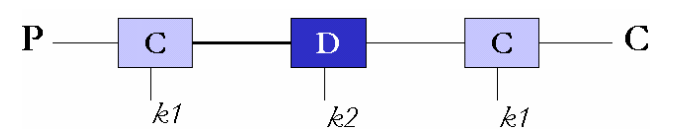
\includegraphics[width=0.5\linewidth]{image.png}
%     \caption{Cifrado de bloque Triple-DES}
%     \label{fig:enter-label}
% \end{figure}
¿Por qué en el modelo de cifrado de bloque de Triple-DES se fortalece el algoritmo a partir del incremento del dominio de la clave y por qué simplemente no se aumenta el tamaño de la misma aplicando una sola vez el algoritmo de cifrado?

\textbf{Respuesta:}

En 3DES se fortalece el algoritmo mediante el incremento del dominio de la clave porque:
\begin{itemize}
    \item Primero que todo aumenta el espacio de claves efectivo sin modificar la estructura básica del algoritmo DES.
    \item Segundo, se tiene una aplicación repetida con diferentes claves para mitigar las vulnerabilidades específicas de DES.
    \item El simple aumento del tamaño de la clave en DES no solucionaría las debilidades estructurales del diseño original.
    \item La arquitectura del DES original está limitada a 56 bits de clave y modificarla para aceptar claves más grandes requeriría rediseñar prácticamente pues todo el algoritmo.
\end{itemize}

\subsection{Literal b}
¿Qué significan las secuencias pseudo-aleatorias en criptografía? ¿Cómo minimizar el riesgo de baja entropía en el cálculo de claves?
\\
\textbf{Respuesta:}

Las secuencias pseudo-aleatorias en criptografía son:
\begin{itemize}
    \item Series de bits generadas por algoritmos deterministas que parecen aleatorias.
    \item Fundamentales para la generación de claves, vectores de inicialización y nonces.
\end{itemize}

Para minimizar el riesgo de baja entropía:
\begin{itemize}
    \item Utilizar fuentes de entropía de alta calidad (ruido térmico, variaciones en hardware, etc.)
    \item Implementar el PRNG criptográficamente seguros (CSPRNG)
    \item Aplicar técnicas de post-procesamiento (función hash) a los datos aleatorios
    \item Realizar pruebas estadísticas de aleatoriedad
\end{itemize}




\subsection{Literal c}
En un cifrador de producto basado en DES/3DES, determine el valor de salida (entero) para la S-Box de la Figura 1, con bloque de entrada 100101, donde $r = b_0b_5$ y $c = b_1b_2b_3b_4$.

\begin{figure}[h]
\centering
\begin{tabular}{|c|c|c|c|c|c|c|c|c|c|c|c|c|c|c|c|c|}
\hline
\multicolumn{17}{|c|}{$S_0$} \\
\hline
& 0 & 1 & 2 & 3 & 4 & 5 & 6 & 7 & 8 & 9 & 10 & 11 & 12 & 13 & 14 & 15 \\
\hline
0 & 14 & 4 & 13 & 1 & 2 & 15 & 11 & 8 & 3 & 10 & 6 & 12 & 5 & 9 & 0 & 7 \\
\hline
1 & 0 & 15 & 7 & 4 & 14 & 2 & 13 & 1 & 10 & 6 & 12 & 11 & 9 & 5 & 3 & 8 \\
\hline
2 & 4 & 1 & 14 & 8 & 13 & 6 & 2 & 11 & 15 & 12 & 9 & 7 & 3 & 10 & 5 & 0 \\
\hline
3 & 15 & 12 & 8 & 2 & 4 & 9 & 1 & 7 & 5 & 11 & 3 & 14 & 10 & 0 & 6 & 13 \\
\hline
\end{tabular}
\caption{S-Box $S_0$ para el cifrador DES}
\end{figure}

\textbf{Solución:}

Tenemos que entonces el bloque de entrada es $100101$

Según el enunciado:
\begin{itemize}
    \item $r = b_0b_5 = (1~1) = 11_2 = 3_{10}$ (la fila 3)
    \item $c = b_1b_2b_3b_4 = (0~0~1~0) = 0010_2 = 2_{10}$ (columna 2)
\end{itemize}

Para obtener el valor de salida, debemos consultar la S-Box $S_0$ en la intersección de la fila 3 y la columna 2:

$$
\begin{array}{|c|c|c|}
\hline
\text{Fila } r & \text{Columna } c & \text{Valor} \\
\hline
3 & 2 & 8 \\
\hline
\end{array}
$$

Por lo tanto el valor que tenemos en la salida (entero) para la S-Box con la entrada $100101$ es 8.


\section{Problema 4 (25\%)}



\subsection{Literal a}
Explique (en pseudo-código) cómo puede implementarse un algoritmo de cifrado de bloque que use mecanismos de sustitución, permutación y condiciones iniciales "fuertes", cálculo de claves. No es necesario ajustarse a estándares ya existentes.

\textbf{Solución}

Para implementar un algoritmo de cifrado por bloques robusto, se requieren varios componentes fundamentales que cumplen propósitos específicos:

\begin{itemize}
    \item \textbf{Entrada y salida}: Mensaje original $M$ y clave secreta $K$ como entradas, texto cifrado $C$ como salida.
    
    \item \textbf{Generación de subclaves}: Derivamos múltiples subclaves a partir de la clave principal porque hay que aumentar la complejidad criptográfica y dificultar ataques de criptoanálisis.
    
    \item \textbf{Condiciones iniciales fuertes}: Aplicamos una permutación inicial para dispersar los bits del mensaje para asegurar que pequeños cambios en la entrada afecten inmediatamente a todo el bloque.
    
    \item \textbf{Proceso de rondas}: Aplicamos múltiples iteraciones de transformaciones para lograr una fuerte difusión y confusión:
        \begin{itemize}
            \item \textbf{Expansión}: Aumentamos el tamaño del estado para crear redundancia y ampliar la superficie de operación.
            
            \item \textbf{Mezcla con subclave}: Combinamos mediante XOR para integrar la información de la clave con el estado actual, creando dependencia de la clave en cada ronda.
            
            \item \textbf{Sustitución}: Aplicamos S-Boxes para introducir no-linealidad, crucial para resistir ataques de criptoanálisis lineal.
            
            \item \textbf{Permutación}: Redistribuimos los bits para garantizar que los cambios en una parte afecten rápidamente a todo el bloque en las siguientes rondas.
        \end{itemize}
\end{itemize}

\textbf{\textit{Pseudo-código:}}

\begin{lstlisting}[basicstyle=\ttfamily\small]
Algoritmo CifradoBloque:
    Entrada: Mensaje M, Clave K
    Salida: Texto cifrado C
    
    // Generación de sub-claves
    SubClaves = GenerarSubClaves(K, NumeroRondas)
    
    // Condiciones iniciales
    EstadoInicial = AplicarPermutacionInicial(M)
    
    // Proceso de rondas
    Estado = EstadoInicial
    Para i desde 1 hasta NumeroRondas:
        // Expansión
        EstadoExpandido = Expansion(Estado)
        
        // Mezcla con subclave
        EstadoMezclado = XOR(EstadoExpandido, SubClaves[i])
        
        // Sustitución (S-Boxes)
        EstadoSustituido = AplicarSustituciones(EstadoMezclado)
        
        // Permutación
        Si i < NumeroRondas entonces:
            Estado = AplicarPermutacion(EstadoSustituido)
        Sino:
            Estado = EstadoSustituido
        Fin Si
    Fin Para
    
    // Permutación final
    C = AplicarPermutacionFinal(Estado)
    
    Retornar C
Fin Algoritmo
\end{lstlisting}

Las funciones auxiliares se implementarían de la siguiente manera:

\begin{itemize}
    \item \textbf{GenerarSubClaves}: Deriva múltiples claves a partir de la clave principal mediante rotaciones, permutaciones y selecciones de bits, garantizando que cada ronda utilice material criptográfico distinto.
    
    \item \textbf{AplicarPermutacionInicial}: Reorganiza los bits del mensaje según una tabla predefinida para asegurar una distribución inicial óptima.
    
    \item \textbf{Expansion}: Aumenta el tamaño del bloque mediante duplicación selectiva de bits para crear más puntos de interacción con la subclave.
    
    \item \textbf{AplicarSustituciones}: Transforma grupos de bits utilizando tablas no lineales (S-Boxes) que mapean entradas a salidas de forma que resistan análisis diferencial y lineal.
    
    \item \textbf{AplicarPermutacion}: Redistribuye los bits resultantes para maximizar el efecto avalancha, donde un cambio en un bit de entrada afecta aproximadamente la mitad de los bits de salida.
    
    \item \textbf{AplicarPermutacionFinal}: Realiza una última reorganización de bits, típicamente inversa a la permutación inicial, para finalizar el proceso de cifrado.
\end{itemize}

La fortaleza de este diseño radica en la combinación de múltiples capas de transformaciones no lineales (sustituciones) con transformaciones lineales (permutaciones), aplicadas repetidamente para crear un cifrado resistente a diversas técnicas de criptoanálisis.





\subsection{Literal b}
Describa brevemente los principales métodos de sustitución y permutación del algoritmo AES/Rijndael e infiera por qué es el estándar de cifrado simétrico más robusto en estos tiempos.
\\
\textbf{Respuesta:}
El algoritmo AES (Advanced Encryption Standard) desarrollado por Vincent Rijmen y Joan Daemen \textit{(basado en Rijndael)}, se estructura en un proceso de cifrado por rondas con operaciones específicas que garantizan tanto la confusión como la difusión de la información. A diferencia de los predecesores como DES, AES no utiliza una estructura Feistel, sino una arquitectura basada en sustitución-permutación (SP) que opera sobre una matriz de estado de 4×4 bytes.

\textbf{Principales métodos de sustitución y permutación en AES:}

\begin{itemize}
    \item \textbf{SubBytes (Sustitución)}: Transformación no lineal que sustituye cada byte del estado por otro valor según una tabla S-Box predefinida. Esta operación:
    \begin{itemize}
        \item Proporciona la no-linealidad necesaria para resistir ataques de criptoanálisis lineal.
        \item Está diseñada matemáticamente para minimizar correlaciones entre bits de entrada y salida.
        \item Se implementa como la inversión en el campo finito GF(2$^8$) seguida de una transformación afín.
    \end{itemize}
    
    \item \textbf{ShiftRows (Permutación)}: Operación donde cada fila de la matriz de estado se desplaza cíclicamente un número diferente de posiciones:
    \begin{itemize}
        \item La primera fila no se desplaza.
        \item La segunda fila se desplaza 1 byte hacia la izquierda.
        \item La tercera fila se desplaza 2 bytes hacia la izquierda.
        \item La cuarta fila se desplaza 3 bytes hacia la izquierda.
        \item Asegura que los bytes de cada columna se dispersen a diferentes columnas, contribuyendo a la difusión entre columnas.
    \end{itemize}
    
    \item \textbf{MixColumns (Difusión)}: Transformación lineal que opera sobre las columnas de la matriz de estado:
    \begin{itemize}
        \item Cada columna se trata como un polinomio de cuatro términos en GF(2$^8$).
        \item Se multiplica módulo $x^4+1$ con un polinomio fijo $a(x) = \{03\}x^3 + \{01\}x^2 + \{01\}x + \{02\}$.
        \item Garantiza que cada byte de salida dependa de todos los bytes de entrada de esa columna.
        \item Proporciona difusión a nivel de columna, complementando la difusión entre columnas de ShiftRows.
    \end{itemize}
    
    \item \textbf{AddRoundKey (Combinación)}: Operación que combina mediante XOR el estado actual con la subclave de ronda:
    \begin{itemize}
        \item Incorpora material de la clave en cada ronda.
        \item Es la única operación que utiliza la clave, proporcionando la seguridad del cifrado.
        \item Simple pero efectiva debido a las propiedades matemáticas del XOR.
    \end{itemize}
\end{itemize}

\textbf{Estructura de rondas en AES:}
\begin{itemize}
    \item \textbf{Ronda inicial}: Aplica únicamente AddRoundKey con la clave original.
    \item \textbf{Rondas principales}: Aplica secuencialmente SubBytes, ShiftRows, MixColumns y AddRoundKey (con 9 rondas para AES-128).
    \item \textbf{Ronda final}: Aplica SubBytes, ShiftRows y AddRoundKey (omite MixColumns).
\end{itemize}

\textbf{AES es considerado el estándar más robusto actualmente porque tiene:}
\begin{itemize}
    \item \textbf{Diseño matemático riguroso}: Basado en principios algebraicos sólidos en campos finitos GF(2$^8$), que proporcionan propiedades criptográficas óptimas.
    
    \item \textbf{Arquitectura innovadora}: A diferencia de los cifradores Feistel tradicionales (como DES, Lucifer, Blowfish), AES procesa el bloque completo en cada ronda, aumentando la difusión y confusión.
    
    \item \textbf{Flexibilidad y escalabilidad}: Permite tamaños de clave de 128, 192 y 256 bits, adaptándose a diferentes requisitos de seguridad y resistiendo ataques cuánticos futuros con claves de mayor longitud.
    
    \item \textbf{Eficiencia computacional}: Diseñado específicamente para optimizar el rendimiento tanto en implementaciones hardware (tarjetas inteligentes con procesadores de 8 bits) como en software (CPUs de 32 bits).
    
    \item \textbf{Resistencia probada}: Ha resistido más de dos décadas de intenso análisis criptográfico sin vulnerabilidades prácticas, mientras que sus contemporáneos como RC2, CAST y IDEA han mostrado debilidades significativas.
    
    \item \textbf{Ausencia de puertas traseras}: A diferencia de algunos algoritmos como Skipjack (propuesto para comunicaciones oficiales en EE.UU.), AES fue seleccionado tras un concurso público abierto y transparente, sin componentes secretos o sospechosos.
    
    \item \textbf{Balance óptimo entre seguridad y rendimiento}: Proporciona un alto nivel de seguridad con una eficiencia computacional excepcional, permitiendo su implementación en dispositivos con recursos limitados.
\end{itemize}

La robustez de AES radica principalmente en su capacidad para crear una fuerte difusión (donde un cambio en un bit de entrada afecta a múltiples bits de salida) y confusión (donde la relación entre la clave y el texto cifrado es compleja), principios fundamentales establecidos por Claude Shannon. Su combinación única de operaciones algebraicas, estructura de rondas y manejo de bytes como elementos de un campo finito lo convierten en un algoritmo matemáticamente sólido y prácticamente invulnerable a los ataques criptoanalíticos conocidos.




\subsection{Literal c}
¿Por qué la operación XOR es usada en los algoritmos criptográficos que operan a nivel de bit y de byte? De un ejemplo.

\textbf{Respuesta:}
La operación XOR (OR exclusivo) es fundamental en algoritmos criptográficos por sus propiedades matemáticas y prácticas:

\begin{itemize}
    \item \textbf{Propiedad de inversión:} $A \oplus B \oplus B = A$ - Esta propiedad permite cifrar y descifrar con la misma operación.
    
    \item \textbf{Distribución uniforme:} Cuando se aplica XOR entre un texto y una clave verdaderamente aleatoria, el resultado no revela patrones estadísticos del texto original.
    
    \item \textbf{Eficiencia computacional:} La operación XOR se implementa con un solo ciclo de reloj en hardware, siendo extremadamente rápida.
    
    \item \textbf{Neutralidad estadística:} No introduce sesgo en la distribución de bits del resultado cuando se aplica con valores aleatorios.
    
    \item \textbf{Propiedad conmutativa:} $A \oplus B = B \oplus A$ - El orden de los operandos no altera el resultado.
\end{itemize}

\textbf{Ejemplo práctico con caracteres ASCII:}

Vamos a cifrar la palabra \texttt{CINCO} usando la clave \texttt{CLAVE} mediante XOR a nivel de byte:

\begin{center}
\begin{tabular}{|c|c|c|c|c|c|}
\hline
\textbf{Operación / Caracter} & \textbf{1} & \textbf{2} & \textbf{3} & \textbf{4} & \textbf{5} \\
\hline

\textbf{Cinco (ASCII)} & \textbf{C} (67) & \textbf{I} (73) & \textbf{N} (78) & \textbf{C} (67) & \textbf{O} (79) \\
\hline
% \textbf{Texto plano (ASCII)} &  \\
% \hline
\textbf{Cinco (binario)} & 01000011 & 01001001 & 01001110 & 01000011 & 01001111 \\
\hline
\textbf{Clave (ASCII)} & C (67) & L (76) & A (65) & V (86) & E (69) \\
\hline
\textbf{Clave (binario)} & 01000011 & 01001100 & 01000001 & 01010110 & 01000101 \\
\hline
\textbf{Cinco XOR Clave} & 00000000 & 00000101 & 00001111 & 00010101 & 00001010 \\
% \hline
% \textbf{Texto cifrado (decimal)} & 0 & 5 & 15 & 21 & 10 \\
% \hline
% \textbf{Texto cifrado (carácter)} & NUL & ENQ & SI & NAK & LF \\
\hline
\end{tabular}
\end{center}

\textbf{Proceso de descifrado:}

Para recuperar el texto original pues aplicamos nuevamente la operación XOR con la misma clave:

\begin{center}
\begin{tabular}{|c|c|c|c|c|c|}
\hline
\textbf{Operación / Caracter} & \textbf{1} & \textbf{2} & \textbf{3} & \textbf{4} & \textbf{5} \\
\hline
% \textbf{Texto cifrado (decimal)} & 0 & 5 & 15 & 21 & 10 \\
% \hline
\textbf{Texto cifrado (binario)} & 00000000 & 00000101 & 00001111 & 00010101 & 00001010 \\
\hline
\textbf{Clave (ASCII)} & C (67) & L (76) & A (65) & V (86) & E (69) \\
\hline
\textbf{Clave (binario)} & 01000011 & 01001100 & 01000001 & 01010110 & 01000101 \\
\hline
\textbf{XOR resultante (binario)} & 01000011 & 01001001 & 01001110 & 01000011 & 01001111 \\
\hline
\textbf{Texto recuperado (decimal)} & 67 & 73 & 78 & 67 & 79 \\
\hline
\textbf{Texto recuperado (carácter)} & C & I & N & C & O \\
\hline
\end{tabular}
\end{center}

\textbf{Demostración de propiedades clave:}

En este ejemplo podemos observar varias propiedades importantes:

\begin{enumerate}
    \item \textbf{Inversión perfecta:} El primer carácter 'C' con valor ASCII 67 se cifra con su homólogo en la clave (también 'C' con valor 67), lo que resulta en 0 (NUL). Esta equivalencia demuestra cómo dos valores idénticos al aplicar XOR se anulan completamente.
    
    \item \textbf{No correlación:} Caracteres similares en el texto plano (las dos 'C' en CINCO) producen diferentes resultados cifrados (0 y 21) debido a las diferentes letras de la clave en esas posiciones ('C' y 'V').
    
    \item \textbf{Difusión:} Un solo bit diferente entre el texto y la clave puede cambiar aproximadamente la mitad de los bits del resultado.
\end{enumerate}

El ejemplo busca mostrar por qué esta operación XOR es el fundamento de muchas primitivas criptográficas, desde el cifrado básico one-time pad hasta operaciones más complejas en cifrados por bloques como AES, donde se utiliza en la fase AddRoundKey para combinar el estado con la subclave de ronda.




% \pagebreak
\subsection*{Muchas gracias por la atención.\\Over V.}

}
% \chapter[Comprehensive User Guide: Instructions for Using the Template]{Comprehensive User Guide Instructions for Using the Template}
% \label{cp:user-guide}

% {
% \parindent0pt

% If you plan to use this template, please read this chapter carefully. It provides all the information you need to effectively use the template, including the mandatory modifications (\textit{e.g.}, title, subtitle, author information) and other configurations that, while not highly recommended, are optional. The template comprises various directories and files, including a total of seven distinct directories and dozens of files. Among these, the most important are \texttt{IPLeiriaMain.tex} and \texttt{IPLeiriaThesis.cls}. Below, \autoref{tab:file-structure} presents the different directories available, along with their descriptions and a check-mark indicating whether you need to access the directory to make changes. Of course, the check-mark indicates that you can make changes to the content, while a hyphen signifies that you should not modify it.

% \begin{table}[!htpb]
%     \setlength{\extrarowheight}{2pt}
%     \caption[Directory structure and file organisation]{Overview of the directory structure in this template.}
%     \label{tab:file-structure}
%     \begin{tabularx}{\textwidth}{lcX}
%         \toprule
%         \\[-1.5\normalbaselineskip]
%         \textbf{Directory} & \textbf{Modifiable} & \textbf{Description} \\ [0em]
%         \midrule
%         \textit{Bibliography} & $\checkmark$ & This folder contains the bibliography file used to manage references throughout the document. \\
%         \textit{Chapters} & $\checkmark$ & Individual chapters of the thesis are organised in this directory, making it easy to work on sections separately. \\
%         \textit{Code} & $\checkmark$ & Code examples and relevant scripts are stored here, supporting the content of the thesis. \\
%         \textit{Configurations} & - & All configuration files required for the template, such as layout and style settings, are placed in this directory. \\
%         \textit{Figures} & $\checkmark$ & All figures and images referenced within the document are stored in this folder for easy access and management. \\
%         \textit{Matter} & - & The front matter of the document, including the cover page, copyright statement, and glossary, is assembled in this directory. \\
%         \textit{Metadata} & $\checkmark$ & This folder holds the metadata file, where key document details such as the author, title, and supervisor can be customised. \\
%         \bottomrule
%     \end{tabularx}
% \end{table}

% It is crucial to note that the files are organized according to a specific naming convention, which must be \textbf{respected} and \textbf{maintained}. The naming convention consists of an ascending two-digit numeric value, followed by a hyphen, and then the file name in capital letters. The name should always aim to be a single word. If more than one word is necessary, they should be separated by a hyphen and capitalised.

% % \begin{verbatim}
% % 00-Abstract.tex
% % 01-Introduction.tex
% % 02-User-Guide.tex
% % ...
% % \end{verbatim}

% \begin{block}[note]
% \textit{While \autoref{tab:file-structure} indicates that the \textit{Matter} directory is not modifiable, two files within that directory should be altered when necessary: \texttt{04-Glossary.tex} and \texttt{05-Acronyms.tex}. Although the names are fairly self-explanatory, these files should contain the glossary and acronyms entries, respectively.}
% \end{block}

% The two files mentioned earlier, \texttt{IPLeiriaMain.tex} and \texttt{IPLeiriaThesis.cls}, should be used with caution. The main file, as the name suggests, is the master file where you will add the necessary chapters to be included in your work. The class file, on the other hand, requires even more caution, and it is not recommended to alter it.

% \section{Template and Class Options}
% \label{sec:class-options}
% The first thing you need to do is specify the options within the \texttt{IPLeiriaMain.tex} file. How do you do that? It's simple. On the very first line, you will find a \texttt{documentclass} command that loads the custom class for this template. In this call, you can pass the options you need. The available options, presented in a key-argument style, are listed in \autoref{tab:template-options}.

% {
% \setlength{\extrarowheight}{-1.75pt}
% \begin{xltabular}{\textwidth}{lX}
% \caption{Class options supported by the template.}
% \label{tab:template-options} \\
% %
% \toprule 
% \multicolumn{1}{l}{\textbf{Options}} & \multicolumn{1}{l}{\textbf{Description}} \\ 
% \midrule
% \endfirsthead
% %
% \multicolumn{2}{c}%
% {{\textit{\bfseries Table \thetable\ continued from previous page.}}} \\
% %
% \toprule 
% \multicolumn{1}{l}{\textbf{Options}} & \multicolumn{1}{l}{\textbf{Description}} \\ 
% \midrule
% \endhead
% %
% \bottomrule
% \addlinespace[1mm]
% \multicolumn{2}{r}%
% {{\textit{Continued on the next page.}}} \\
% \endfoot
% \bottomrule
% \endlastfoot

% \textbf{school=OPT} & \textbf{Choosing a school and its corresponding logo.} \\
% \multirow[t]{2}{*}{\footnotesize{\textit{estg, esecs, esslei, esad, estm}}} & \footnotesize{\textit{$\Rightarrow$ Default: school=estg}} \\
% & \footnotesize{\textit{This option only modifies the school name and the corresponding logo, which will be displayed on the cover and front page.}} \\[1.70em]

% \textbf{language=OPT} & \textbf{Language preference selection.} \\
% \footnotesize{\textit{portuguese, english}} & \footnotesize{\textit{$\Rightarrow$ Default: language=english}} \\[0.85em]
        
% \textbf{chapterstyle=OPT} & \textbf{Selection of a cover design style.} \\
% \multirow[t]{2}{*}{\footnotesize{\textit{classic, modern, fancy}}} & \footnotesize{\textit{$\Rightarrow$ Default: chapterstyle=classic}} \\
% & \footnotesize{\textit{This option modifies the appearance of the chapter, including its title and numbering style. Explore the available styles and apply the one you prefer.}} \\[1.70em]

% \textbf{coverstyle=OPT} & \textbf{Choosing a style for the chapter.} \\
% \multirow[t]{3}{*}{\footnotesize{\textit{classic, bw}}} & \footnotesize{\textit{$\Rightarrow$ Default: coverstyle=classic}} \\
% & \footnotesize{\textit{classic $\rightarrow$ Put the cover on in the original red.}} \\
% & \footnotesize{\textit{bw $\rightarrow$ Make the cover black and white.}} \\

% \pagebreak

% \textbf{docstage=OPT} & \textbf{Choosing a stage for you document.} \\
% \multirow[t]{3}{*}{\footnotesize{\textit{final, working}}} & \footnotesize{\textit{$\Rightarrow$ Default: docstage=final}} \\
% & \footnotesize{\textit{final $\rightarrow$ Assumes this is the final version of the document.}} \\
% & \footnotesize{\textit{working $\rightarrow$ It assumes the document is a work in progress.}} \\[.3em]

% \textbf{media=OPT} & \textbf{Project media type.} \\
% \multirow[t]{3}{*}{\footnotesize{\textit{paper, screen}}} & \footnotesize{\textit{$\Rightarrow$ Default: media=paper}} \\
% & \footnotesize{\textit{paper $\rightarrow$ Blank pages will appear between sections.}} \\
% & \footnotesize{\textit{screen $\rightarrow$ Blank pages will not appear between sections.}} \\[.3em]

% \textbf{colorlink=OPT} & \textbf{Main theme color.} \\
% \multirow[t]{2}{*}{\footnotesize{\textit{color}}} & \footnotesize{\textit{$\Rightarrow$ Default: colorlink=black}} \\
% & \footnotesize{\textit{This option requires a valid color name. Refer to the xcolor manual (subsection 4.2) to select a valid color.}} \\
% \end{xltabular}
% }

% \begin{block}[tip]
% \textit{Although the default option for \texttt{linkcolor} is \texttt{black}, it is highly advisable to use \texttt{red!45!black} instead. The same applies to \texttt{coverstyle}, for which it is preferred to use the \texttt{classic} option.}
% \end{block}

% % \begin{block}[warning]
% % \textit{If any option or argument is passed and it does not exist, an error or a warning will be raised, respectively. Please pay attention to warnings and strive to keep the template and/or your document free of warnings.}
% % \end{block}

% After setting the options within the main class, you're ready to proceed with the metadata customisation. How can you do that? Please refer to \autoref{sec:metadata}.

% \section{Metadata Customisation}
% \label{sec:metadata}
% While options like language and school can be passed as arguments to the main class, other options, such as author and title, need to be defined manually. Since this template supports a wide range of metadata options, a dedicated file is provided for this purpose. The file is located at \texttt{Metadata/Metadata.tex} and contains the metadata variables you can modify, along with comments explaining each variable and whether it is mandatory for the document. To omit a variable, simply comment it out. Below, \autoref{tab:metadata} presents all the available metadata variables, their GET command, and whether they are mandatory. The GET command is important if you want to automatically retrieve the name or information stored in a given variable.

% \begin{longtable}[c]{llc}
% \caption{Metadata variables within the template.}
% \label{tab:metadata} \\
% \toprule
% \textbf{Variable} & \textbf{Macro Commands} & \textbf{Mandatory} \\ \midrule
% \endfirsthead
% %
% \multicolumn{3}{c}%
% {{\textit{\bfseries Table \thetable\ continued from previous page.}}} \\
% %
% \toprule
% \textbf{Variable} & \textbf{Macro Commands} & \textbf{Mandatory} \\ \midrule
% \endhead
% %
% \bottomrule
% %
% \addlinespace[1mm]
% \multicolumn{3}{r}%
% {{\textit{Continued on the next page.}}} \\
% \endfoot
% %
% \bottomrule
% %
% \endlastfoot
% %
% Title            & \verb|\GetTitle|         & $\checkmark$ \\
% Subtitle         & \verb|\GetSubtitle|      & $\checkmark$ \\
% University       & \verb|\GetUniversity|    & $\checkmark$ \\
% School           & \verb|\GetSchool|        & $\checkmark$ \\
% Department       & \verb|\GetDepartment|    & $\checkmark$ \\
% Degree           & \verb|\GetDegree|        & $\checkmark$ \\
% Course           & \verb|\GetCourse|        & -            \\
% Local and date   & \verb|\Get\|          & $\checkmark$  \\ 
% Academic year    & \verb|\GetAcademicYear|  & $\checkmark$ \\ 

% Thesis type (\scriptsize{\textit{Dissertation, Project or Internship}}) & \verb|\GetThesisType| & $\checkmark$ \\

% First author name           & \verb|\GetFirstAuthor|        & $\checkmark$ \\
% First author identification & \verb|\GetFirstAuthorNumber|  & $\checkmark$ \\ 

% Second author name           & \verb|\GetSecondAuthor|          & - \\
% Second author identification & \verb|\GetSecondAuthorNumber|    & - \\ 

% Third author name           & \verb|\GetThirdAuthor|        & - \\
% Third author identification & \verb|\GetThirdAuthorNumber|  & - \\ 

% Supervisor name                  & \verb|\GetSupervisor|        & $\checkmark$ \\
% Supervisor e-mail                & \verb|\GetSupervisorMail|    & $\checkmark$ \\
% Supervisor title and affiliation & \verb|\GetSupervisorTitle|   & $\checkmark$ \\ 

% Co-supervisor name                  & \verb|\GetCoSupervisor|       & - \\
% Co-supervisor e-mail                & \verb|\GetCoSupervisorMail|   & - \\
% Co-supervisor title and affiliation & \verb|\GetCoSupervisorTitle|  & - \\ 

% Second co-supervisor name                   & \verb|\GetSecCoSupervisor|      & - \\
% Second co-supervisor e-mail                 & \verb|\GetSecCoSupervisorMail|  & - \\
% Second co-supervisor title and affiliation  & \verb|\GetSecCoSupervisorTitle| & - \\
% \end{longtable}

% If, by any chance, \textbf{you want to add more options}, please contact me by opening an issue in the official GitHub repository or via the email provided in this document.

% \section{Custom Commands}
% Within this template, some custom commands are also available for your use. For example, if you are writing your thesis and want to add a to-do note, you can easily insert a block with the option \verb|todo|, as follows: \verb|\begin{block}[todo]|. This will insert a to-do block with a style similar to Markdown. Other available options are: \verb|tip|, \verb|warning|, and \verb|note|. Below is a visual example for each one.

% \vspace{.875em}
% \begin{tcbraster}[
%     raster columns=2, 
%     raster equal height, 
%     nobeforeafter, 
%     raster column skip=2cm
% ]
% \begin{block}[todo]
%     \textit{This is a to-do block.}
% \end{block}
% \begin{block}[tip]
%     \textit{This is a tip block.}
% \end{block}
% \end{tcbraster}

% \begin{tcbraster}[
%     raster columns=2, 
%     raster equal height, 
%     nobeforeafter, 
%     raster column skip=2cm
% ]
% \begin{block}[warning]
%     \textit{This is a warning block.}
% \end{block}
% \begin{block}[note]
%     \textit{This is a note block.}
% \end{block}
% \end{tcbraster}
% \vspace{.875em}

% Another custom command that can come in handy is \verb|\myuline{TEXT}|, which creates a visually improved underline. The default \LaTeX~underline is not ideal because it sits directly below the bottom margin of the word, increasing the line height of the paragraph. This new command provides a \myuline{better} and more \myuline{stylish} underline.

% \section{Custom Chapter Insertion}
% As stated before, to use this template, you need to do three things: set the appropriate options in the document class (refer to \autoref{sec:class-options}), update the document metadata (refer to \autoref{sec:metadata}), and create and import your custom chapters. To create and import a custom chapter, follow these steps: \(i\) create a TeX file under the Chapters directory that follows the predefined naming convention, and \(ii)\) include it in the main file using the command \verb|\include{CHAPTER}|. And voilà, your first chapter is ready!
% }
% \chapter[Essential LaTeX Tutorial: Fundamentals and Key Concepts]{Essential LaTeX Tutorial Fundamentals and Key Concepts}
% \label{cp:latex-tutorial}

% {
% \parindent0pt

% In this chapter, we will introduce the \LaTeX~working environment, highlighting the basic essentials you will need to produce your thesis. First of all, \LaTeX~(pronounced ``LAY-tek'' or ``LAH-tek'') is a tool for creating professional-quality documents. Unlike \textit{What You See Is What You Get} editors like Microsoft Word, \LaTeX~uses plain text files containing both content and formatting commands. These files are processed by a TeX engine, which interprets the commands to produce a polished, typeset PDF. This approach lets you focus on your content, leaving the precise formatting and layout to \LaTeX~and the TeX engine, ensuring a professional result every time. While this chapter will introduce you to some important functionalities of \LaTeX~, please take the time to learn \LaTeX~from the beginning. You can always refer to the Overleaf \href{https://www.overleaf.com/learn/latex/Learn_LaTeX_in_30_minutes}{Learn LaTeX} series for guidance.

% % Moreover, if you are spending an enormous amount of time writing your thesis, it's better to use a proper tool where you don't need to worry about professional layout but can focus solely on the content.

% \section{Citations}
% \label{sec:citations}
% We present two distinct approaches for citing entries in the bibliography. The first method involves in-text citations, executed using \verb|\citet{ENTRY}|, while the second method employs \verb|\citep{ENTRY}| for citations within a paragraph. Below is an example demonstrating both usages. It's essential to note that you can cite multiple works within the same citation environment. To achieve this, you should use the following format: \verb|\citep{ENTRY1, ENTRY2, ...}|. It is also possible to cite only the title of the work or the author of the same. To do this, please use \verb|\citetitle{ENTRY}| for title citations and \verb|\citeauthor{ENTRY}| for author citations.

% \begin{block}[tip]
% \textit{Proper citations play a crucial role in academic writing, serving as the foundation for credibility, transparency, and the advancement of knowledge. They are a fundamental aspect of responsible scholarly writing. Please ensure accurate and appropriate citations.}
% \end{block}

% \noindent\textbf{Example:} A novel signature scheme is introduced, along with an implementation of the Diffie-Hellman key distribution scheme that accomplishes a public key cryptosystem \citep{Elgamal1985}. According to \citet{Elgamal1985}, a new signature scheme that accomplishes a public key cryptosystem is introduced (...) This template was created by \citeauthor{IPLeiriaThesis}, with the title \citetitle{IPLeiriaThesis}.

% \section{References}
% Much like citations, it is advisable to employ references in your document for citing crucial elements such as chapters, sections, figures, or tables. To reference these elements, begin by creating a label. This label can be generated using \verb|\label{TEXT}|, and it should be positioned within the element you intend to refer to. Once the element is created, you can utilise \verb|\ref{LABEL}| to generate an in-text reference. \textbf{We strongly recommend using} \verb|\autoref{LABEL}|. This command automatically creates a custom link with color corresponding to the type of element being referred to. For instance, a chapter reference will appear like this: \autoref{cp:introduction}, rather than simply Chapter \ref{cp:introduction}. 

% \begin{block}[tip]
% \textit{Properly referencing elements within the document, such as \textbf{chapters, sections, figures, tables, or listings}, is crucial.}
% \end{block}

% \section{Glossary and Acronyms}
% The document includes both a glossary and an acronym list, accessible at the beginning of the document. You can create a new entry in either the \verb|Matter/02-Glossary| or \verb|Matter/03-Acronyms| sections, depending on the type of entry you intend to add. Once the entry is created, you can reference it using \verb|\gls{ENTRY}| for glossary entries. For acronym entries, there are two ways to reference them. The first method, \verb|\acrfull{ENTRY}|, should be used the first time the acronym appears in the text as it automatically provides the definition in-text. Subsequently, to refer to the acronym without repeating its meaning, use \verb|\acrshort{ENTRY}|.

% \vspace{.875em}
% \textbf{Example:} Utilising \Gls{latex} for \Gls{maths} is essential (...). It is advisable to seek both the \acrfull{gcd} and \acrfull{lcm} because (...). Subsequently, with the aid of \acrshort{gcd} and \acrshort{lcm}, we can (...).

% \section{Figures}
% In \LaTeX, integrating figures is a straightforward process. To insert them, you should utilise the environment \verb|\begin{figure}|. You can customise the \verb|width| parameter according to your requirements, but it is crucial to select a high-quality figure when inserting it into your documents. It is equally crucial to furnish a well-crafted caption. If necessary, consider including citations or references to indicate the figure's origin. The caption environment is denoted as \verb|\caption{TEXT}|. To generate a smaller caption for the Table of Figures, be sure to utilise the format \verb|\caption[SMALL_TEXT]{BIG_TEXT}|. By following the aforementioned tips, we can create a figure as demonstrated in \autoref{fig:figure-01}.

% \begin{figure}[!htpb]
%     \centering
%     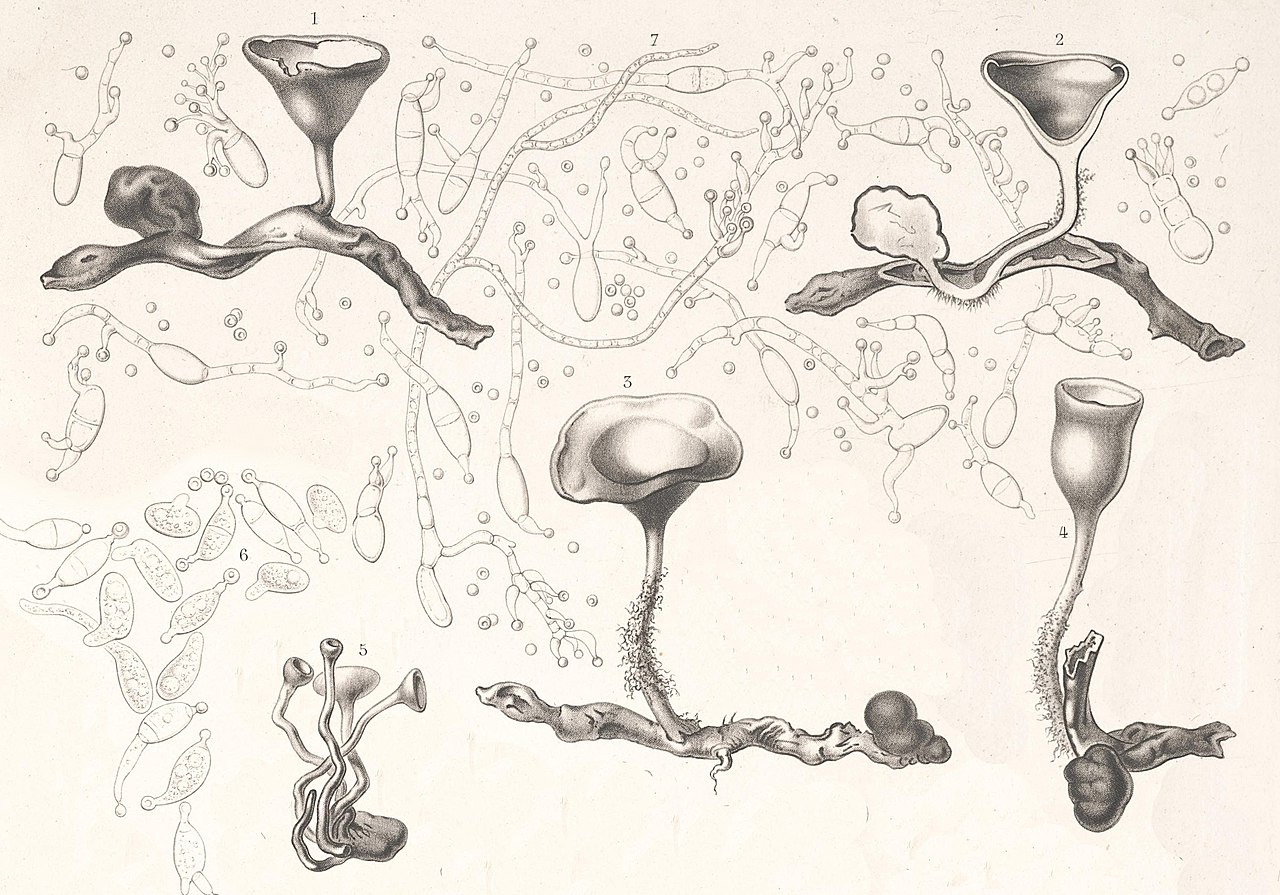
\includegraphics[width=\linewidth]{Figures/PezizaTuberosa.jpg}
%     \caption[Illustration of the fungus Dumontinia tuberosa.]{Illustration of the fungus Dumontinia tuberosa by physician, mycologist, and illustrator Charles Tulasne (1816–1884) in the book Selecta Fungorum Carpologia (1861–65). (Name of the original work: Peziza tuberosa parasite on Anemone nemorosa).}
%     \label{fig:figure-01}
% \end{figure}

% For the purpose of comparing or for other reasons, you can insert side-by-side figures using both the \verb|\begin{figure}| and \verb|\begin{subfigure}| environments. You can also refer to the sub-figure as \autoref{fig:figure-02.1} and \autoref{fig:figure-02.2}.

% \begin{figure}[!htpb]
%     \centering
%     \begin{subfigure}{0.45\textwidth}
%         \centering
%         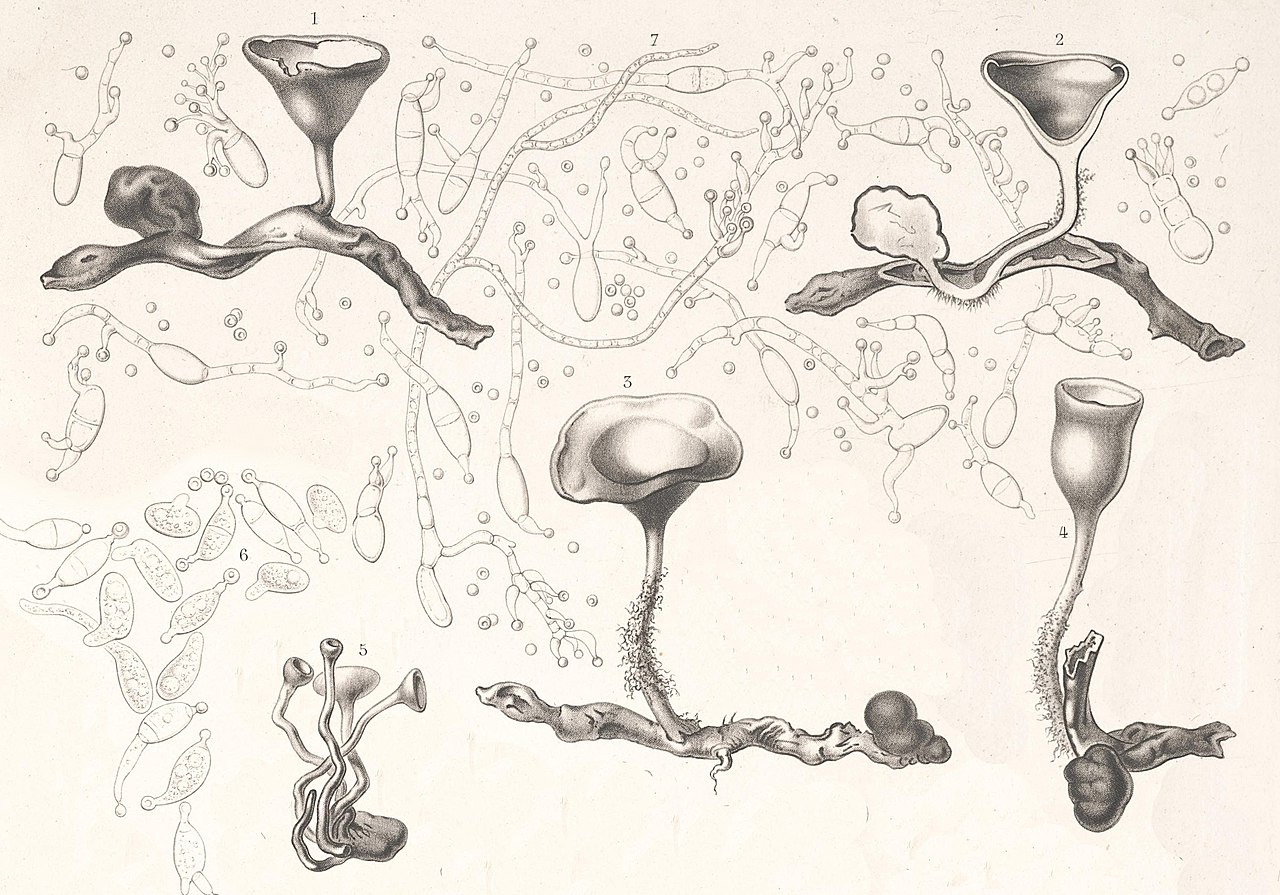
\includegraphics[width=0.9\textwidth]{Figures/PezizaTuberosa.jpg}
%         \caption{Caption for figure 1.}
%         \label{fig:figure-02.1}
%     \end{subfigure}
%     \hspace{.5cm} % Adjust the space as needed.
%     \begin{subfigure}{0.45\textwidth}
%         \centering
%         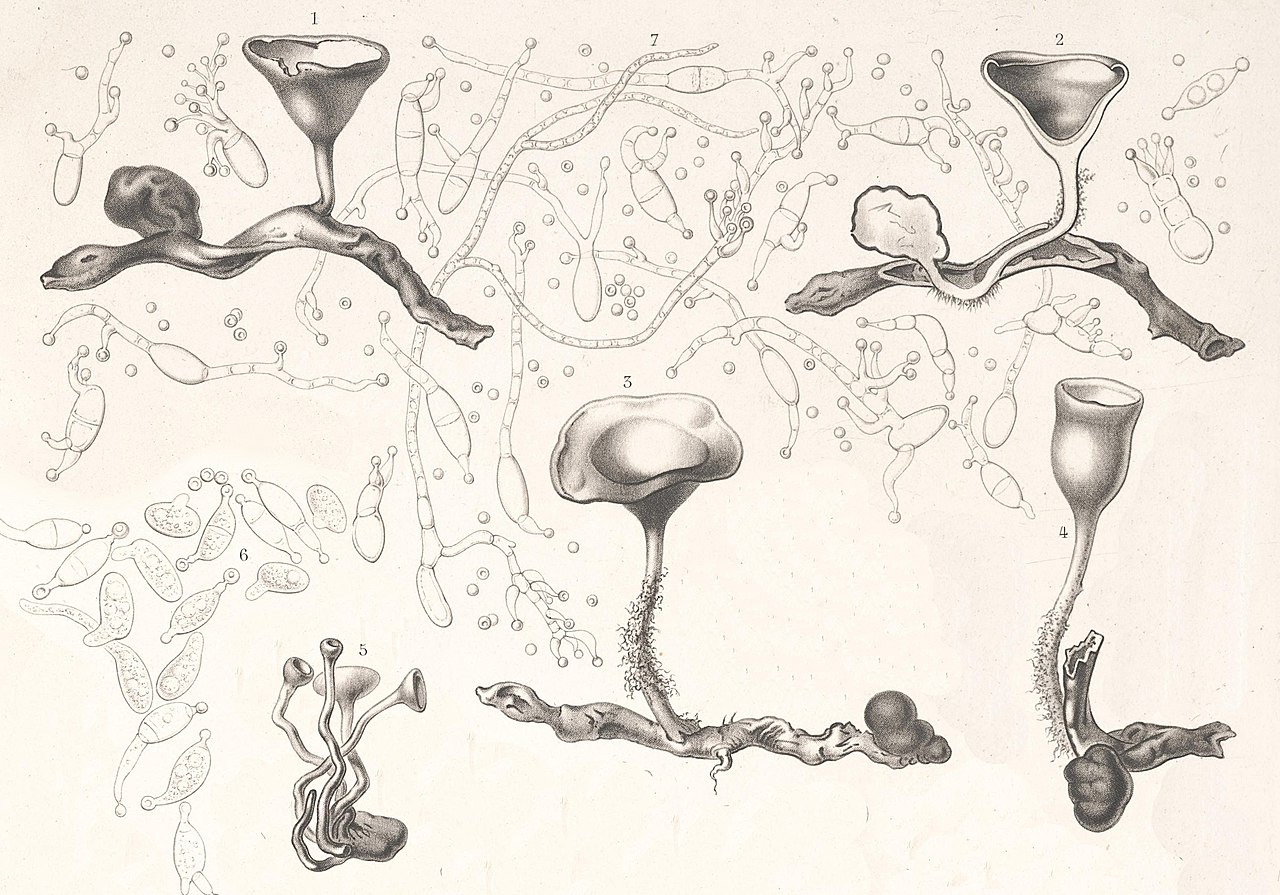
\includegraphics[width=0.9\textwidth]{Figures/PezizaTuberosa.jpg}
%         \caption{Caption for figure 2.}
%         \label{fig:figure-02.2}
%     \end{subfigure}
%     \caption{Overall caption of the figure.}
%     \label{fig:figure-02}
% \end{figure}

% \section{Tables}
% Tables are vital for presenting findings effectively. This chapter explores techniques for conveying information through tables using various template environments. Defining tables in \LaTeX\ seems complex, but this template simplifies the process.

% \begin{block}[tip]
% \textit{Prior to showcasing the different table environments, it's crucial to note that each one must be enclosed within a \texttt{\textbackslash begin\{table\}} environment. Additionally, it is recommended to utilise the \texttt{[!htpb]} float options for improved document placement. \textbf{This advice should be taken into consideration when positioning figures as well}.}
% \end{block}

% \subsection{Tabular Environment}
% The conventional \verb|\begin{tabular}| environment enables you to create a simple yet elegant table. \autoref{tab:table-01} is generated using a centering environment for added emphasis. It also incorporates the \verb|booktab| configuration for a more sophisticated table style.

% \begin{table}[!htpb]
%     \caption{A table showcasing the usage of the tabular environment.}
%     \label{tab:table-01}
%     \centering
%     \begin{tabular}{llc}
%         \toprule
%         \textbf{Header 01} & \textbf{Header 02} & \textbf{Header 03} \\ 
%         \midrule
%         Lorem Ipsum         & Pharetra Dolor    & $\checkmark$  \\
%         Amet Consectetuer   & Curabitur Aliquet & -             \\
%         Praesent Mauris     & Praesent Libero   & $\checkmark$  \\
%         \bottomrule
%     \end{tabular}
% \end{table}

% \subsection{Tabularx Environment}
% Employ the \verb|\begin{tabularx}| package to construct a table featuring automatically expanding multi-columns. To achieve this automatic behaviour for multi-columns, you can use the following environment: \verb|\begin{tabularx}{\textwidth}{lX}|, where \verb|X| is the column that will function as a multi-column. \autoref{tab:table-02} showcases the usage of the \verb|begin{tabularx}| environment.
% %Take note that we substitute \verb|X| in place of \verb|l| or \verb|c|, explicitly indicating that the column will function as a multi-column, occupying the entire available space.

% \begin{table}[!htpb]
%     \caption{A table showcasing the usage of the tabularx environment.}
%     \label{tab:table-02}
%     \begin{tabularx}{\textwidth}{lX}
%         \toprule
%         \textbf{Header 01} & \textbf{Header 02} \\ 
%         \midrule
%         Foo Bar Baz & Quisque cursus, metus vitae pharetra auctor, sem massa mattis sem, at interdum magna augue eget diam. \\
%         Ipsum Dolor & Vestibulum ante ipsum primis in faucibus orci luctus et ultrices posuere cubilia Curae; Curabitur aliquet quam id dui. \\
%         Dolor Sit & Phasellus condimentum elementum justo, quis interdum est sagittis ac. Vestibulum non arcu sit amet justo lobortis semper. \\
%         Amet Consectetuer & Integer nec odio praesent libero sed cursus ante dapibus diam sed nisi vestibulum non arcu. \\
%         Consectetuer Adipiscing & Nulla quis sem at nibh elementum imperdiet. Duis sagittis ipsum. Praesent mauris. \\
%         \bottomrule
%     \end{tabularx}
% \end{table}

% \subsection{Longtable Environment}
% At times, when dealing with exceptionally lengthy tables, it becomes necessary to split them across multiple pages. In \LaTeX, this can be achieved using the \verb|\begin{longtable}| environment. This environment is slightly more complex than others, as you need to define the header twice: once for the initial appearance of the table and again for when the table spans additional pages. This repeated header ensures the reader can correctly identify the columns on subsequent pages. Feel free to consult \autoref{tab:table-03} for a detailed demonstration of how the \verb|longtable| environment works.

% \begin{longtable}[c]{llll}
% \caption{A table showcasing the usage of the longtable environment.}
% \label{tab:table-03} \\
% \toprule
% \textbf{Names} & \textbf{E-Mails} & \textbf{Job/Role} \\ \midrule
% \endfirsthead
% %
% \multicolumn{4}{c}%
% {{\textit{\bfseries Table \thetable\ continued from previous page.}}} \\
% \toprule
% \textbf{Names} & \textbf{E-Mails} & \textbf{Job/Role} \\ \midrule
% \endhead
% %
% \bottomrule
% \addlinespace[1mm]
% \multicolumn{4}{r}%
% {{\textit{Continued on the next page.}}} \\
% \endfoot
% \bottomrule
% %
% \endlastfoot
% %
% Alice Johnson & alice.johnson@email.com & Project Manager \\
% Bob Thompson & bob.thompson@email.com & Data Analyst \\
% Charlie Davis & charlie.davis@email.com & Marketing Specialist \\
% David Miller & david.miller@email.com & QA Tester \\
% Emily White & emily.white@email.com & Graphic Designer \\
% Frank Martin & frank.martin@email.com & HR Coordinator \\
% Grace Turner & grace.turner@email.com & Financial Analyst \\
% Henry Lee & henry.lee@email.com & System Administrator \\
% Ivy Carter & ivy.carter@email.com & Customer Support \\
% Jack Wilson & jack.wilson@email.com & Frontend Developer \\
% Jane Reed & jane.reed@email.com & UX Designer \\
% Kevin Evans & kevin.evans@email.com & Product Manager \\
% Linda Adams & linda.adams@email.com & Accountant \\
% Mike Hill & mike.hill@email.com & Network Engineer \\
% Nina Garcia & nina.garcia@email.com & Business Analyst \\
% Oliver Smith & oliver.smith@email.com & Sales Representative \\
% Pamela Turner & pamela.turner@email.com & Legal Counsel \\
% Quincy Brown & quincy.brown@email.com & IT Consultant \\
% Rachel Moore & rachel.moore@email.com & Content Writer \\
% Samuel White & samuel.white@email.com & Research Scientist \\ 
% Amy Harris & amy.harris@email.com & Digital Strategist \\
% Brian Cook & brian.cook@email.com & Operations Manager \\
% Catherine Ross & catherine.ross@email.com & Brand Manager \\
% Daniel Green & daniel.green@email.com & Database Administrator \\
% Emma Taylor & emma.taylor@email.com & Social Media Manager \\
% Felix Carter & felix.carter@email.com & Compliance Officer \\
% Gloria Scott & gloria.scott@email.com & Procurement Specialist \\
% Harold Bennett & harold.bennett@email.com & DevOps Engineer \\
% Isla Cooper & isla.cooper@email.com & User Researcher \\
% James Black & james.black@email.com & Mobile App Developer \\
% Katie Brown & katie.brown@email.com & UI Designer \\
% Leo Perez & leo.perez@email.com & Scrum Master \\
% Megan Clark & megan.clark@email.com & Event Coordinator \\
% Nathan Ward & nathan.ward@email.com & Security Analyst \\
% Olivia Harris & olivia.harris@email.com & Corporate Trainer \\
% Paul King & paul.king@email.com & Territory Manager \\
% Queen Foster & queen.foster@email.com & Paralegal \\
% Rebecca Adams & rebecca.adams@email.com & Copy Editor \\
% Steven Martin & steven.martin@email.com & Robotics Engineer \\
% \end{longtable}

% \subsection{Complex Tables}
% Creating intricate tables in \LaTeX\ can be a somewhat challenging task. Therefore, we highly recommend using the \href{https://www.tablesgenerator.com/}{Table Generator}. With this tool, you can design your table with the desired style and then easily copy and paste it into your document. This approach simplifies the process and helps ensure the accurate representation of complex tables in your \LaTeX\ document. However, it's crucial to keep in mind that a table should be easily comprehensible for the reader and should not be overly complex. \textbf{The complexity of a table may impede understanding.} For example, \autoref{tab:table-04} presents a table with intricate details.

% \begin{table}[!htpb]
%     \caption{A table showcasing the usage of the complex tables.}
%     \label{tab:table-04}
%     \centering
%     \begin{tabular}{lcc}
%         \toprule
%         \multirow{2}{*}{\textbf{Component}} & \multicolumn{2}{c}{\textbf{Specifications}} \\
%         \cmidrule(lr){2-3}
%         & \textbf{Characteristic} & \textbf{Supported} \\
%         \midrule
%         \multirow{4}{*}{CPU} & Core Count (e.g., 8 Cores) & $\checkmark$ \\
%         & Clock Speed (e.g., 3.6 GHz) & $\checkmark$ \\
%         & Hyper-Threading & $\checkmark$ \\
%         & Integrated Graphics & - \\
%         \midrule
%         \multirow{4}{*}{GPU} & CUDA Cores (e.g., 5120) & $\checkmark$ \\
%         & Base Clock (e.g., 1.5 GHz) & $\checkmark$ \\
%         & Ray Tracing Support & $\checkmark$ \\
%         & Multi-GPU Support (SLI/CrossFire) & - \\
%         \midrule
%         \multirow{4}{*}{Memory} & Type (e.g., DDR5, GDDR6) & $\checkmark$ \\
%         & Capacity (e.g., 16 GB) & $\checkmark$ \\
%         & Memory Bandwidth (e.g., 448 GB/s) & $\checkmark$ \\
%         & ECC Support & - \\
%         \midrule
%         \multirow{3}{*}{Motherboard Features} & PCIe 5.0 Support & $\checkmark$ \\
%         & Wi-Fi 6E & $\checkmark$ \\
%         & Thunderbolt 4 & - \\
%         \bottomrule
%     \end{tabular}
% \end{table}

% \section{Lists}
% Creating lists in \LaTeX\ is straightforward, offering various options to suit your needs. You can generate a bullet list using \verb|\begin{itemize}|, or opt for a numbered list with \verb|\begin{enumerate}|. Below is an example with the \verb|\begin{itemize}| environment.

% \begin{itemize}
%   \item List entries start with the \verb|\item| command.
%   \item Individual entries are indicated with a black dot, a so-called bullet.
%   \item The text in the entries may be of any length.
% \end{itemize}

% As mentioned earlier, you can generate a numbered list using the \verb|\begin{enumerate}| environment. Here is an example:

% \begin{enumerate}
%   \item Items are numbered automatically.
%   \item The numbers start at 1 with each use of the \verb|enumerate| environment.
%   \item Another entry in the list.
% \end{enumerate}

% You can also nest list entries by creating a list inside another list of the same type. Here is an example:

% \begin{enumerate}
%     \item First level item
%     \item First level item
%     \begin{enumerate}
%         \item Second level item
%         \item Second level item
%     \begin{enumerate}
%         \item Third level item
%         \item Third level item
%     \end{enumerate}
%     \end{enumerate}
% \end{enumerate}

% \begin{block}[tip]
% \textit{Please note that the labels change automatically regardless of the environment being the same for every list. \textbf{This demonstrates that there's no need to worry about changing the environment for something different.}}
% \end{block}

% You can also modify the label of your list to something entirely different that suits your needs. To accomplish this, insert a new \verb|\item| and enclose your desired label in square brackets. For example, \verb|\item[!]| will result in an exclamation point as your new label. Below are some examples of modified labels.

% \begin{itemize}
%   \item This is my first point
%   \item Another point I want to make 
%   \item[!] A point to exclaim something!
%   \item[$\blacksquare$] Make the point fair and square.
%   \item[] A blank label?
% \end{itemize}

% Finally, you can create a description list. Unlike having a bullet point or a numbered label, a description list enables you to use custom descriptions that suit your list. In the example below, there are three \verb|\item| entries: one without a label, and two with descriptions.

% \begin{description}
%     \item[Item 1:] This is the first item with a description.
%     \item[Item 2:] Another item with a different description.
%     \item An item without a specific label.
% \end{description}

% \section{Code Listings}
% At times, you may want to include source code from your programs and applications within your document. To achieve this, you can use two nested environments: \verb|\begin{listing}| to create a listing with both caption and label, and \verb|\begin{minted}| for code highlighting. \autoref{listing:c-code} provides an example of a source code in C.

% \begin{listing}[!htpb]
% \caption{Hello world in C.}
% \label{listing:c-code}
% \begin{minted}{c}
% #include <stdio.h>
% int main() {
%    printf("Hello, World!"); /* printf() outputs the quoted string */
%    return 0;
% }
% \end{minted}
% \end{listing}

% The code mentioned above was inserted into the document. However, an alternative approach is to input your code from an external file. To do so, you just need to use the command \verb|\inputminted{CODE_LANGUAGE}{FILE}|. Of course, you should place that command inside of the \verb|\begin{listing}| environment. \autoref{listing:haskell-code} illustrates an example of Haskell source code that has been input from an external file.

% \begin{listing}[!htpb]
% \caption{Factorial in Haskell.}
% \label{listing:haskell-code}
% \inputminted{haskell}{Code/Factorial.hs}
% \end{listing}

% In some cases, when you simply want to highlight a specific command, it's recommended not to use \verb|listing| or \verb|minted|. Instead, you should utilise the \verb|\verb| command for inline highlighting or the \verb|\begin{verbatim}| environment for longer sections of highlighted code. An example of a lengthy \verb|verbatim| section is provided below, demonstrating how to create a \verb|listing| with an input code:

% \begin{verbatim}
% \begin{listing}[!htpb]
%     \inputminted{CODE_LANGUAGE}{FILE}
%     \caption{TEXT}
%     \label{TEXT}
% \end{listing}
% \end{verbatim}

% Sometimes it is necessary to display longer code that occupies more than one page. For this purpose, please use the environment \verb|\begin{longlisting}|. This environment will easily break your code into multiple pages for better readability without you worrying about the size of your code. An example is shown below in \autoref{listing:lisp-code}.

% \begin{longlisting}
% \caption{A sample of functions in Lisp.}
% \label{listing:lisp-code}
% \begin{minted}{lisp}
% (defun factorial (n)
%   "Calculate the factorial of a number."
%   (if (zerop n)
%       (* n (factorial (1- n)))))

% (defun fibonacci (n)
%   "Calculate the nth Fibonacci number."
%   (cond ((zerop n) 0)
%         ((= n 1) 1)
%         (t (+ (fibonacci (1- n)) (fibonacci (- n 2))))))

% (defun gcd (a b)
%   "Calculate the greatest common divisor of a and b."
%   (if (zerop b)
%       a
%       (gcd b (mod a b))))

% (defun primes-up-to (limit)
%   "Return a list of all prime numbers up to LIMIT."
%   (let ((primes '()))
%     (loop for i from 2 to limit
%           unless (some (lambda (p) (zerop (mod i p))) primes)
%           do (push i primes))
%     (nreverse primes)))

% (defun example-function (x)
%   "An example function to demonstrate Lisp capabilities."
%   (let ((result (list (factorial x)
%                       (fibonacci x)
%                       (gcd x 10)
%                       (primes-up-to x))))
%     (format t "Factorial of ~A: ~A~%" x (factorial x))
%     (format t "Fibonacci of ~A: ~A~%" x (fibonacci x))
%     (format t "GCD of ~A and 10: ~A~%" x (gcd x 10))
%     (format t "Primes up to ~A: ~A~%" x (primes-up-to x))
%     result))

% (example-function 10)
% \end{minted}
% \end{longlisting}

% \section{Equations}
% When writing equations and other mathematical expressions, \LaTeX~is a powerful and versatile tool. You can enter a formula in inline mode using the environment \verb|\(FORMULA\)| or use \verb|\begin{equation}| to display it in ``math mode'' with numbering. If you prefer not to display the equation number, you can use the environment \verb|\[FORMULA\]|.

% \vspace{.875em}
% \textbf{Example:} In physics, the mass-energy equivalence is expressed by the equation \(E=mc^2\), discovered in 1905 by Albert Einstein. In natural units ($c = 1$), the formula (\ref{eq:equation-01}) expresses the identity:

% \begin{equation}
% \label{eq:equation-01}
% E=m
% \end{equation}

% \textbf{Example:} Below is a equation -- \textit{without numbering} -- for the regularised loss function in supervised learning, combining the average prediction loss over the training dataset and an $L_2$ regularisation term to prevent overfitting:

% \[
% \mathcal{L}(\boldsymbol{\theta}) = \frac{1}{N} \sum_{i=1}^{N} \ell(y_i, f(\mathbf{x}_i; \boldsymbol{\theta})) + \lambda \|\boldsymbol{\theta}\|_2^2
% \]

% Equations can be a bit challenging to create, so we advise using an online editor, like the \href{https://latexeditor.lagrida.com/}{LaTeX Equation Editor}. Simply build your formulas there and copy and paste them into your document, either inline or in a math block, as shown above.

% \section{Footnotes}
% Sometimes it is important to present information that is not central to the main text in a footnote. In \LaTeX\, this can be easily achieved using the command \verb|\footnote{TEXT}|. The text will appear at the bottom of the page\footnote{This is a simple footnote.}.

% If you want to use footnotes within tables, it is best to reconsider, as \LaTeX\ does not provide an easy way to handle them. Instead, you can place a ``*'' wherever you want the footnote reference to appear. Then, below the table \textbf{but before ending the table environment}, place the ``*'' along with the footnote text. This will create a similar footnote, but it will appear below the table rather than at the bottom of the page.
% }

%%% Bibliography %%%
% \renewcommand{\refname}{Bibliography}
% \printbibliography[title={\refname},heading=bibintoc]

%%% Appendices: Work that *YOU* Developed %%%
\appendix
% \ifthenelse{\equal{\LanguageOption}{portuguese}}{
%     \addtocontents{toc}{\protect\contentsline{chapter}{Apêndices}{}{}}
% }{
%     \addtocontents{toc}{\protect\contentsline{chapter}{Appendices}{}{}}
% }

% % \ifthenelse{\equal{\MediaOption}{paper}}{\blankpage}{\clearpage}
% % \begin{center}
% %     \crimsonfont
% %     \thispagestyle{empty}
        
% %     \vspace*{\fill}
% %     \ifthenelse{\equal{\LanguageOption}{portuguese}}{%
% %         {\LARGE\fontsize{26}{26}\selectfont\textcolor{maincolor}{Apêndices}\par}
% %     }{%
% %         {\LARGE\fontsize{26}{26}\selectfont\textcolor{maincolor}{Appendices}\par}
% %     }
% %     \vspace*{\fill}
% % \end{center}
% \MediaOptionLogicBlank
% \chapter{Showcasing the First Appendix}
% \guideinfo{Appendices contain supplementary material \textbf{created by the author} that enhances the reader’s understanding of the dissertation while not being essential for following the primary narrative. These sections often include detailed tables, figures, complex calculations, or materials like survey questions and interview transcripts produced in the course of the research. The appendices allow readers to explore the research in greater detail, offering a deeper insight into methods and findings without interrupting the main body of work.}
% % Recommended dimensions for a landscape layout; adjust as needed.
% \begin{landscapemode}{297mm}{420mm}
%     \chapter{Showcasing the Second Appendix}
%     \blindtext[5]
% \end{landscapemode}

%%% Annexes: Work that *YOU DID NOT* Develop %%%
% \ifthenelse{\equal{\LanguageOption}{portuguese}}{
%     \addtocontents{toc}{\protect\contentsline{chapter}{Anexos}{}{}}
% }{
%     \addtocontents{toc}{\protect\contentsline{chapter}{Annexes}{}{}}
% }

% \setcounter{chapter}{11} % To start at the "L" chapter.
% \MediaOptionLogicAnnexes
% \begin{center}
%     \crimsonfont
%     \thispagestyle{empty}
        
%     \vspace*{\fill}
%     \ifthenelse{\equal{\LanguageOption}{portuguese}}{%
%         {\LARGE\fontsize{26}{26}\selectfont\textcolor{maincolor}{Anexos}\par}
%     }{%
%         {\LARGE\fontsize{26}{26}\selectfont\textcolor{maincolor}{Annexes}\par}
%     }
%     \vspace*{\fill}
% \end{center}
% \MediaOptionLogicBlank
% \chapter{Showcasing the First Annex}
% \guideinfo{Annexes are supplementary sections in a dissertation that provide additional information or external documents not essential to the main arguments but that support or complement the research. Unlike appendices, \textbf{annexes generally contain material that was not developed by the author}, such as reports, legal documents, or published datasets from external sources. This information is placed separately to keep the main content concise, allowing readers access to relevant external references without disrupting the dissertation's flow.}

%%% Back Page %%%
% \ifthenelse{\equal{\MediaOption}{paper}}{\blankpage}{}

% \clearpage
% \null
% \thispagestyle{empty}

% \ifthenelse{\equal{\CoverOption}{classic}}{
%     \newcommand\BackgroundPicBackPage{%
%     \put(0,0){%
%     \parbox[b][\paperheight]{\paperwidth}{%
%     \vfill
%     \centering
%     
\includegraphics[width=\paperwidth,height=\paperheight,keepaspectratio]{Figures/Theme/Back-Page-BG.pdf}%
%     \vfill
%     }}}
% }{
%     \newcommand\BackgroundPicBackPage{%
%     \put(0,0){%
%     \parbox[b][\paperheight]{\paperwidth}{%
%     \vfill
%     \centering
%     
\includegraphics[width=\paperwidth,height=\paperheight,keepaspectratio]{Figures/Theme/Back-Page-BG-W.pdf}%
%     \vfill
%     }}}
% }

% \AddToShipoutPictureBG*{\BackgroundPicBackPage}

% \newgeometry{margin=1.98cm, top=1.47cm, bottom=1.47cm}
% \noindent\clearpage
% \restoregeometry

\end{document}